\documentclass[twoside]{book}

% Packages required by doxygen
\usepackage{fixltx2e}
\usepackage{calc}
\usepackage{doxygen}
\usepackage[export]{adjustbox} % also loads graphicx
\usepackage{graphicx}
\usepackage[utf8]{inputenc}
\usepackage{makeidx}
\usepackage{multicol}
\usepackage{multirow}
\PassOptionsToPackage{warn}{textcomp}
\usepackage{textcomp}
\usepackage[nointegrals]{wasysym}
\usepackage[table]{xcolor}

% Font selection
\usepackage[T1]{fontenc}
\usepackage[scaled=.90]{helvet}
\usepackage{courier}
\usepackage{amssymb}
\usepackage{sectsty}
\renewcommand{\familydefault}{\sfdefault}
\allsectionsfont{%
  \fontseries{bc}\selectfont%
  \color{darkgray}%
}
\renewcommand{\DoxyLabelFont}{%
  \fontseries{bc}\selectfont%
  \color{darkgray}%
}
\newcommand{\+}{\discretionary{\mbox{\scriptsize$\hookleftarrow$}}{}{}}

% Page & text layout
\usepackage{geometry}
\geometry{%
  a4paper,%
  top=2.5cm,%
  bottom=2.5cm,%
  left=2.5cm,%
  right=2.5cm%
}
\tolerance=750
\hfuzz=15pt
\hbadness=750
\setlength{\emergencystretch}{15pt}
\setlength{\parindent}{0cm}
\setlength{\parskip}{3ex plus 2ex minus 2ex}
\makeatletter
\renewcommand{\paragraph}{%
  \@startsection{paragraph}{4}{0ex}{-1.0ex}{1.0ex}{%
    \normalfont\normalsize\bfseries\SS@parafont%
  }%
}
\renewcommand{\subparagraph}{%
  \@startsection{subparagraph}{5}{0ex}{-1.0ex}{1.0ex}{%
    \normalfont\normalsize\bfseries\SS@subparafont%
  }%
}
\makeatother

% Headers & footers
\usepackage{fancyhdr}
\pagestyle{fancyplain}
\fancyhead[LE]{\fancyplain{}{\bfseries\thepage}}
\fancyhead[CE]{\fancyplain{}{}}
\fancyhead[RE]{\fancyplain{}{\bfseries\leftmark}}
\fancyhead[LO]{\fancyplain{}{\bfseries\rightmark}}
\fancyhead[CO]{\fancyplain{}{}}
\fancyhead[RO]{\fancyplain{}{\bfseries\thepage}}
\fancyfoot[LE]{\fancyplain{}{}}
\fancyfoot[CE]{\fancyplain{}{}}
\fancyfoot[RE]{\fancyplain{}{\bfseries\scriptsize Generated by Doxygen }}
\fancyfoot[LO]{\fancyplain{}{\bfseries\scriptsize Generated by Doxygen }}
\fancyfoot[CO]{\fancyplain{}{}}
\fancyfoot[RO]{\fancyplain{}{}}
\renewcommand{\footrulewidth}{0.4pt}
\renewcommand{\chaptermark}[1]{%
  \markboth{#1}{}%
}
\renewcommand{\sectionmark}[1]{%
  \markright{\thesection\ #1}%
}

% Indices & bibliography
\usepackage{natbib}
\usepackage[titles]{tocloft}
\setcounter{tocdepth}{3}
\setcounter{secnumdepth}{5}
\makeindex

% Hyperlinks (required, but should be loaded last)
\usepackage{ifpdf}
\ifpdf
  \usepackage[pdftex,pagebackref=true]{hyperref}
\else
  \usepackage[ps2pdf,pagebackref=true]{hyperref}
\fi
\hypersetup{%
  colorlinks=true,%
  linkcolor=blue,%
  citecolor=blue,%
  unicode%
}

% Custom commands
\newcommand{\clearemptydoublepage}{%
  \newpage{\pagestyle{empty}\cleardoublepage}%
}

\usepackage{caption}
\captionsetup{labelsep=space,justification=centering,font={bf},singlelinecheck=off,skip=4pt,position=top}

%===== C O N T E N T S =====

\begin{document}

% Titlepage & ToC
\hypersetup{pageanchor=false,
             bookmarksnumbered=true,
             pdfencoding=unicode
            }
\pagenumbering{roman}
\begin{titlepage}
\vspace*{7cm}
\begin{center}%
{\Large eco-\/bot \\[1ex]\large 3.\+0 }\\
\vspace*{1cm}
{\large Generated by Doxygen 1.8.11}\\
\end{center}
\end{titlepage}
\clearemptydoublepage
\tableofcontents
\clearemptydoublepage
\pagenumbering{arabic}
\hypersetup{pageanchor=true}

%--- Begin generated contents ---
\chapter{R\+E\+A\+D\+ME}
\label{md_README}
\hypertarget{md_README}{}


\href{https://travis-ci.org/Prasheel24/Object-Collector-Robot}{\tt } \href{https://coveralls.io/github/Prasheel24/Object-Collector-Robot?branch=master}{\tt } \href{https://github.com/Prasheel24/Object-Collector-Robot/blob/master/LICENSE}{\tt }

\subsection*{Authors}


\begin{DoxyItemize}
\item {\bfseries Raj Prakash Shinde} \href{https://github.com/RajPShinde}{\tt Git\+Hub} ~\newline
I am a Masters in Robotics Engineering student at the University of Maryland, College Park. My primary area of interest are Legged Robotics and Automation.
\item {\bfseries Prasheel Renkuntla} \href{https://github.com/Prasheel24}{\tt Git\+Hub} ~\newline
I am a Master\textquotesingle{}s in Robotics Engineering student at the University of Maryland, College Park. My primary area of interest is in Vision integrated Robot Systems.
\end{DoxyItemize}

\subsection*{Overview}

This is R\+OS Package developed for A\+C\+ME Robotics to demonstrate the functionality of their new eco-\/bot.

\subsection*{Sprint Planning and Discussion}

Sprint-\/ \href{https://docs.google.com/document/d/1_uG7fMXPrtZlpRLsgD74NdLRX3DKDXxCicppZWBDNvQ}{\tt Link}

\subsection*{Agile Iterative Process Log}

Log-\/ \href{https://docs.google.com/spreadsheets/d/1DkxCx4_GxvRXjRTTrmgZvdOQ4z0DMrpGEavg439tQak}{\tt Link}

\subsection*{Dependencies}


\begin{DoxyEnumerate}
\item Ubuntu 16.\+04
\item C++ 11/14/17
\item R\+OS Kinetic
\item Turtlebot stack ~\newline
 Install by running following command 
\begin{DoxyCode}
1 sudo apt-get install ros-kinetic-turtlebot-gazebo ros-kinetic-turtlebot-apps
       ros-kinetic-turtlebot-rviz-launchers
\end{DoxyCode}

\end{DoxyEnumerate}

\subsection*{Build}

Steps to build 
\begin{DoxyCode}
1 mkdir -p ~/catkin\_ws/src
2 cd ~/catkin\_ws/
3 catkin\_make
4 source devel/setup.bash
5 cd src/
6 git clone https://github.com/Prasheel24/Object-Collector-Robot
7 cd ~/catkin\_ws/
8 catkin\_make
\end{DoxyCode}
 \subsection*{Run}

{\bfseries Generate Map} ~\newline
 Open a new Terminal 
\begin{DoxyCode}
1 source devel/setup.bash
2 roslaunch ecobot TurtlebotMapping.launch
\end{DoxyCode}
 {\bfseries Save Map to Directory} ~\newline
 Open a new Terminal 
\begin{DoxyCode}
1 rosrun map\_server map\_saver map:=/robot\_1/map -f CollectorSpace
\end{DoxyCode}
 {\bfseries Collect Garbage} ~\newline
 Open a new Terminal 
\begin{DoxyCode}
1 source devel/setup.bash
2 roslaunch ecobot TurtlebotCollect.launch
\end{DoxyCode}


\subsection*{References}


\begin{DoxyItemize}
\item \href{http://wiki.ros.org/}{\tt http\+://wiki.\+ros.\+org/}
\item \href{http://wiki.ros.org/rrt_exploration}{\tt http\+://wiki.\+ros.\+org/rrt\+\_\+exploration}
\item \href{http://wiki.ros.org/navigation/Tutorials/Writing%20A%20Global%20Path%20Planner%20As%20Plugin%20in%20ROS}{\tt http\+://wiki.\+ros.\+org/navigation/\+Tutorials/\+Writing\%20\+A\%20\+Global\%20\+Path\%20\+Planner\%20\+As\%20\+Plugin\%20in\%20\+R\+OS}
\item \href{https://www.geeksforgeeks.org/a-search-algorithm/}{\tt https\+://www.\+geeksforgeeks.\+org/a-\/search-\/algorithm/}
\end{DoxyItemize}

\subsection*{Contributions}


\begin{DoxyItemize}
\item $\ast$$\ast$\+R\+RT Exploration Package-\/$\ast$$\ast$ {\itshape H. Umari and S. Mukhopadhyay, \char`\"{}\+Autonomous robotic exploration based on multiple rapidly-\/exploring randomized trees,\char`\"{} 2017 I\+E\+E\+E/\+R\+SJ International Conference on Intelligent Robots and Systems (I\+R\+OS), Vancouver, BC, 2017, pp. 1396-\/1402.} {\itshape doi\+: 10.\+1109/\+I\+R\+OS.2017.\+8202319} {\itshape keywords\+: \{edge detection;mobile robots;multi-\/agent systems;navigation;path planning;random processes;robot vision;trees (mathematics);efficient robotic exploration;three-\/dimensional space;autonomous robotic exploration;randomized trees;efficient robotic navigation;autonomous exploration strategies;edge detection;dimensional exploration;multiple Rapidly-\/exploring Random Trees;R\+RT algorithm;Robot Operating System framework;frontier detection;image processing;Detectors;Image edge detection;Robot sensing systems;Path planning;Navigation\},} U\+RL\+: \href{http://ieeexplore.ieee.org/stamp/stamp.jsp?tp=&arnumber=8202319&isnumber=8202121}{\tt http\+://ieeexplore.\+ieee.\+org/stamp/stamp.\+jsp?tp=\&arnumber=8202319\&isnumber=8202121}
\item $\ast$$\ast$\+Logo -\/$\ast$$\ast$ \href{https://www.flaticon.com/authors/nhor-phai}{\tt https\+://www.\+flaticon.\+com/authors/nhor-\/phai}
\end{DoxyItemize}

\subsection*{Disclaimer}


\begin{DoxyCode}
1 BSD 3-Clause License
2 
3 Copyright (c) 2019, Raj Shinde
4 Copyright (c) 2019, Prasheel Renkuntla
5 All rights reserved.
6 
7 Redistribution and use in source and binary forms, with or without
8 modification, are permitted provided that the following conditions are met:
9 
10 1. Redistributions of source code must retain the above copyright notice, this
11    list of conditions and the following disclaimer.
12 
13 2. Redistributions in binary form must reproduce the above copyright notice,
14    this list of conditions and the following disclaimer in the documentation
15    and/or other materials provided with the distribution.
16 
17 3. Neither the name of the copyright holder nor the names of its
18    contributors may be used to endorse or promote products derived from
19    this software without specific prior written permission.
20 
21 THIS SOFTWARE IS PROVIDED BY THE COPYRIGHT HOLDERS AND CONTRIBUTORS "AS IS"
22 AND ANY EXPRESS OR IMPLIED WARRANTIES, INCLUDING, BUT NOT LIMITED TO, THE
23 IMPLIED WARRANTIES OF MERCHANTABILITY AND FITNESS FOR A PARTICULAR PURPOSE ARE
24 DISCLAIMED. IN NO EVENT SHALL THE COPYRIGHT HOLDER OR CONTRIBUTORS BE LIABLE
25 FOR ANY DIRECT, INDIRECT, INCIDENTAL, SPECIAL, EXEMPLARY, OR CONSEQUENTIAL
26 DAMAGES (INCLUDING, BUT NOT LIMITED TO, PROCUREMENT OF SUBSTITUTE GOODS OR
27 SERVICES; LOSS OF USE, DATA, OR PROFITS; OR BUSINESS INTERRUPTION) HOWEVER
28 CAUSED AND ON ANY THEORY OF LIABILITY, WHETHER IN CONTRACT, STRICT LIABILITY,
29 OR TORT (INCLUDING NEGLIGENCE OR OTHERWISE) ARISING IN ANY WAY OUT OF THE USE
30 OF THIS SOFTWARE, EVEN IF ADVISED OF THE POSSIBILITY OF SUCH DAMAGE.
\end{DoxyCode}
 
\chapter{Namespace Index}
\section{Namespace List}
Here is a list of all namespaces with brief descriptions\+:\begin{DoxyCompactList}
\item\contentsline{section}{\hyperlink{namespaceastar__plugin}{astar\+\_\+plugin} }{\pageref{namespaceastar__plugin}}{}
\end{DoxyCompactList}

\chapter{Hierarchical Index}
\section{Class Hierarchy}
This inheritance list is sorted roughly, but not completely, alphabetically\+:\begin{DoxyCompactList}
\item Base\+Global\+Planner\begin{DoxyCompactList}
\item \contentsline{section}{astar\+\_\+plugin\+:\+:A\+Star\+Planner}{\pageref{classastar__plugin_1_1_a_star_planner}}{}
\end{DoxyCompactList}
\item \contentsline{section}{Collector}{\pageref{class_collector}}{}
\item \contentsline{section}{Grid\+Square}{\pageref{class_grid_square}}{}
\item \contentsline{section}{Navigate\+Robot}{\pageref{class_navigate_robot}}{}
\item \contentsline{section}{Randomizer}{\pageref{class_randomizer}}{}
\item \contentsline{section}{Spawn\+Collect}{\pageref{class_spawn_collect}}{}
\end{DoxyCompactList}

\chapter{Class Index}
\section{Class List}
Here are the classes, structs, unions and interfaces with brief descriptions\+:\begin{DoxyCompactList}
\item\contentsline{section}{\hyperlink{classastar__plugin_1_1_a_star_planner}{astar\+\_\+plugin\+::\+A\+Star\+Planner} }{\pageref{classastar__plugin_1_1_a_star_planner}}{}
\item\contentsline{section}{\hyperlink{class_collector}{Collector} }{\pageref{class_collector}}{}
\item\contentsline{section}{\hyperlink{class_grid_square}{Grid\+Square} }{\pageref{class_grid_square}}{}
\item\contentsline{section}{\hyperlink{class_navigate_robot}{Navigate\+Robot} }{\pageref{class_navigate_robot}}{}
\item\contentsline{section}{\hyperlink{class_randomizer}{Randomizer} }{\pageref{class_randomizer}}{}
\item\contentsline{section}{\hyperlink{class_spawn_collect}{Spawn\+Collect} }{\pageref{class_spawn_collect}}{}
\end{DoxyCompactList}

\chapter{File Index}
\section{File List}
Here is a list of all files with brief descriptions\+:\begin{DoxyCompactList}
\item\contentsline{section}{include/\hyperlink{collector_8hpp}{collector.\+hpp} \\*Final Project -\/ ecobot (A trash Collecting Robot) }{\pageref{collector_8hpp}}{}
\item\contentsline{section}{include/\hyperlink{grid_square_8hpp}{grid\+Square.\+hpp} }{\pageref{grid_square_8hpp}}{}
\item\contentsline{section}{include/\hyperlink{navigate_robot_8hpp}{navigate\+Robot.\+hpp} }{\pageref{navigate_robot_8hpp}}{}
\item\contentsline{section}{include/\hyperlink{path_planner_8hpp}{path\+Planner.\+hpp} }{\pageref{path_planner_8hpp}}{}
\item\contentsline{section}{include/\hyperlink{randomizer_8hpp}{randomizer.\+hpp} \\*Final Project -\/ ecobot (A trash Collecting Robot) }{\pageref{randomizer_8hpp}}{}
\item\contentsline{section}{include/\hyperlink{spawn_collect_8hpp}{spawn\+Collect.\+hpp} \\*Final Project -\/ ecobot (A trash Collecting Robot) }{\pageref{spawn_collect_8hpp}}{}
\item\contentsline{section}{src/\hyperlink{collector_8cpp}{collector.\+cpp} \\*Final Project -\/ ecobot (A trash Collecting Robot) }{\pageref{collector_8cpp}}{}
\item\contentsline{section}{src/\hyperlink{grid_square_8cpp}{grid\+Square.\+cpp} \\*Final Project -\/ ecobot (A trash Collecting Robot) }{\pageref{grid_square_8cpp}}{}
\item\contentsline{section}{src/\hyperlink{src_2main_8cpp}{main.\+cpp} }{\pageref{src_2main_8cpp}}{}
\item\contentsline{section}{src/\hyperlink{navigate_robot_8cpp}{navigate\+Robot.\+cpp} \\*Final Project -\/ ecobot (A trash Collecting Robot) }{\pageref{navigate_robot_8cpp}}{}
\item\contentsline{section}{src/\hyperlink{path_planner_8cpp}{path\+Planner.\+cpp} \\*Final Project -\/ ecobot (A trash Collecting Robot) }{\pageref{path_planner_8cpp}}{}
\item\contentsline{section}{src/\hyperlink{randomizer_8cpp}{randomizer.\+cpp} \\*Final Project -\/ ecobot (A trash Collecting Robot) }{\pageref{randomizer_8cpp}}{}
\item\contentsline{section}{src/\hyperlink{spawn_collect_8cpp}{spawn\+Collect.\+cpp} \\*Final Project -\/ ecobot (A trash Collecting Robot) }{\pageref{spawn_collect_8cpp}}{}
\item\contentsline{section}{test/\hyperlink{test_2main_8cpp}{main.\+cpp} }{\pageref{test_2main_8cpp}}{}
\item\contentsline{section}{test/\hyperlink{test_grid_square_8cpp}{test\+Grid\+Square.\+cpp} \\*Final Project -\/ ecobot (A trash Collecting Robot) }{\pageref{test_grid_square_8cpp}}{}
\item\contentsline{section}{test/\hyperlink{test_navigate_robot_8cpp}{test\+Navigate\+Robot.\+cpp} \\*Final Project -\/ ecobot (A trash Collecting Robot) }{\pageref{test_navigate_robot_8cpp}}{}
\item\contentsline{section}{test/\hyperlink{test_path_planner_8cpp}{test\+Path\+Planner.\+cpp} }{\pageref{test_path_planner_8cpp}}{}
\item\contentsline{section}{test/\hyperlink{test_randomizer_8cpp}{test\+Randomizer.\+cpp} \\*Final Project -\/ ecobot (A trash Collecting Robot) }{\pageref{test_randomizer_8cpp}}{}
\item\contentsline{section}{test/\hyperlink{test_spawn_collect_8cpp}{test\+Spawn\+Collect.\+cpp} \\*Final Project -\/ ecobot (A trash Collecting Robot) }{\pageref{test_spawn_collect_8cpp}}{}
\end{DoxyCompactList}

\chapter{Namespace Documentation}
\hypertarget{namespaceastar__plugin}{}\section{astar\+\_\+plugin Namespace Reference}
\label{namespaceastar__plugin}\index{astar\+\_\+plugin@{astar\+\_\+plugin}}
\subsection*{Classes}
\begin{DoxyCompactItemize}
\item 
class \hyperlink{classastar__plugin_1_1_a_star_planner}{A\+Star\+Planner}
\end{DoxyCompactItemize}

\chapter{Class Documentation}
\hypertarget{classastar__plugin_1_1_a_star_planner}{}\section{astar\+\_\+plugin\+:\+:A\+Star\+Planner Class Reference}
\label{classastar__plugin_1_1_a_star_planner}\index{astar\+\_\+plugin\+::\+A\+Star\+Planner@{astar\+\_\+plugin\+::\+A\+Star\+Planner}}


{\ttfamily \#include $<$path\+Planner.\+hpp$>$}

Inheritance diagram for astar\+\_\+plugin\+:\+:A\+Star\+Planner\+:\begin{figure}[H]
\begin{center}
\leavevmode
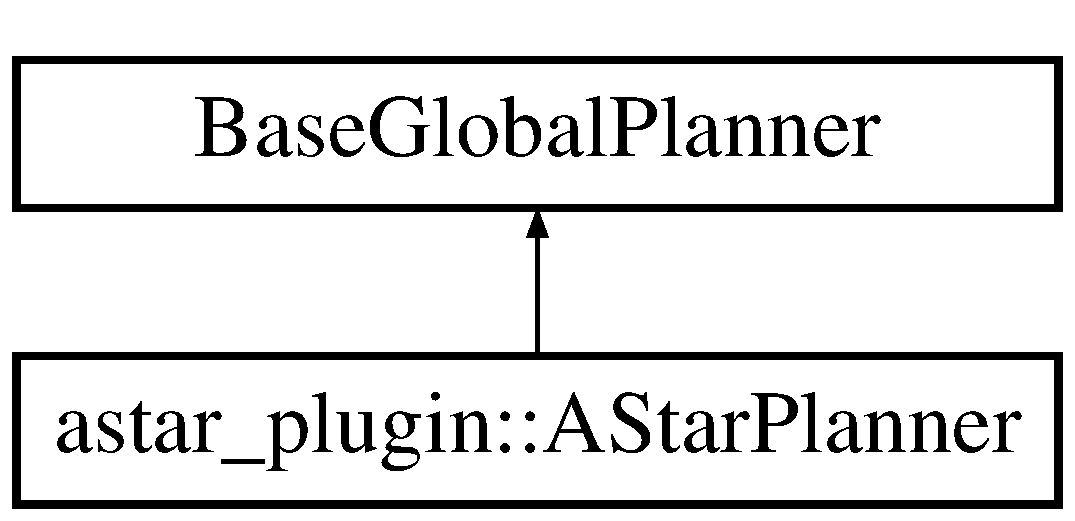
\includegraphics[height=2.000000cm]{classastar__plugin_1_1_a_star_planner}
\end{center}
\end{figure}
\subsection*{Public Member Functions}
\begin{DoxyCompactItemize}
\item 
\hyperlink{classastar__plugin_1_1_a_star_planner_a709090708527da7d103f7c9373f4b651}{A\+Star\+Planner} ()
\begin{DoxyCompactList}\small\item\em Constructor of class A\+Star planner. \end{DoxyCompactList}\item 
\hyperlink{classastar__plugin_1_1_a_star_planner_a79cd3d4231e807ccc04f70d1e4ecd837}{A\+Star\+Planner} (ros\+::\+Node\+Handle \&)
\begin{DoxyCompactList}\small\item\em Overloaded constructor to call ros node handle. \end{DoxyCompactList}\item 
\hyperlink{classastar__plugin_1_1_a_star_planner_a6eaf79c8595c501e03117436fd499e42}{A\+Star\+Planner} (std\+::string name, costmap\+\_\+2d\+::\+Costmap2\+D\+R\+OS $\ast$\hyperlink{classastar__plugin_1_1_a_star_planner_a1be22c40d97241edb0a60b7bd3c332f3}{costmap\+\_\+ros})
\begin{DoxyCompactList}\small\item\em Overloaded constructor to initialise 2D cost map. \end{DoxyCompactList}\item 
void \hyperlink{classastar__plugin_1_1_a_star_planner_abd555da48b7cb20f1fef16962ac0a71c}{initialize} (std\+::string name, costmap\+\_\+2d\+::\+Costmap2\+D\+R\+OS $\ast$\hyperlink{classastar__plugin_1_1_a_star_planner_a1be22c40d97241edb0a60b7bd3c332f3}{costmap\+\_\+ros})
\begin{DoxyCompactList}\small\item\em Function inherited from base class to initialise map. \end{DoxyCompactList}\item 
bool \hyperlink{classastar__plugin_1_1_a_star_planner_a0452b64fca4b454fad7da2249494a9fd}{make\+Plan} (const geometry\+\_\+msgs\+::\+Pose\+Stamped \&start, const geometry\+\_\+msgs\+::\+Pose\+Stamped \&goal, std\+::vector$<$ geometry\+\_\+msgs\+::\+Pose\+Stamped $>$ \&plan)
\begin{DoxyCompactList}\small\item\em Function to make a plan to reach the goal. \end{DoxyCompactList}\item 
std\+::vector$<$ int $>$ \hyperlink{classastar__plugin_1_1_a_star_planner_a70e9cb8c51872dd8f83d1ae4a7006c62}{run\+A\+Star} (int start\+Cell, int goal\+Cell)
\begin{DoxyCompactList}\small\item\em Function to run astar algorithm. \end{DoxyCompactList}\item 
std\+::vector$<$ int $>$ \hyperlink{classastar__plugin_1_1_a_star_planner_a65c23083aa562f0ce8a881d26fb020a7}{find\+Path} (int start\+Cell, int goal\+Cell, std\+::vector$<$ float $>$ g\+\_\+score)
\begin{DoxyCompactList}\small\item\em Function to find path to reach the goal. \end{DoxyCompactList}\item 
std\+::vector$<$ int $>$ \hyperlink{classastar__plugin_1_1_a_star_planner_aae75ccdcf38f6cd848d024a8aebc0bc0}{construct\+Path} (int start\+Cell, int goal\+Cell, std\+::vector$<$ float $>$ g\+\_\+score)
\begin{DoxyCompactList}\small\item\em Function to construct a path to reach the goal. \end{DoxyCompactList}\item 
std\+::vector$<$ float $>$ \hyperlink{classastar__plugin_1_1_a_star_planner_a875990bd4b8b9ab17855ce54b4df4780}{get\+Map\+Coordinates} (float x, float y)
\begin{DoxyCompactList}\small\item\em Function to get map coordinates. \end{DoxyCompactList}\item 
float \hyperlink{classastar__plugin_1_1_a_star_planner_a18fac92699522fa76a2add6ea75fa6fc}{calculate\+H\+Cell\+Score} (int cell\+Index, int cell\+Square)
\begin{DoxyCompactList}\small\item\em Function to calculate H cell score. \end{DoxyCompactList}\item 
int \hyperlink{classastar__plugin_1_1_a_star_planner_aa54d997cd223de69fb7a37a79dc5cd1c}{calculate\+Cell\+Index} (int i, int j)
\begin{DoxyCompactList}\small\item\em Function to calculate cell index. \end{DoxyCompactList}\item 
int \hyperlink{classastar__plugin_1_1_a_star_planner_a660c014cd14a8de3080b138b44f5437e}{get\+Cell\+Row\+Index} (int index)
\begin{DoxyCompactList}\small\item\em Function to get Cell Row index. \end{DoxyCompactList}\item 
int \hyperlink{classastar__plugin_1_1_a_star_planner_a7242cadadc720feb8af97bc9f427f53c}{get\+Cell\+Col\+Index} (int index)
\begin{DoxyCompactList}\small\item\em Function to get Cell Column index. \end{DoxyCompactList}\item 
bool \hyperlink{classastar__plugin_1_1_a_star_planner_a29d81e8f4ac6191296d5c180be9ac8ae}{is\+Cell\+Free} (int cell\+Index)
\begin{DoxyCompactList}\small\item\em Function to check if the cell is free. \end{DoxyCompactList}\item 
bool \hyperlink{classastar__plugin_1_1_a_star_planner_ae8f5105e002f679874c3d55815fe30ad}{is\+Cell\+Free} (int i, int j)
\begin{DoxyCompactList}\small\item\em Overloaded function to check if cell is free. \end{DoxyCompactList}\item 
float \hyperlink{classastar__plugin_1_1_a_star_planner_ad07f32fd3a1e44ef3bb9bb1e59237023}{get\+Move\+To\+Cell\+Cost} (int cell\+Index1, int cell\+Index2)
\begin{DoxyCompactList}\small\item\em Function to get moving cost to a cell. \end{DoxyCompactList}\item 
float \hyperlink{classastar__plugin_1_1_a_star_planner_a2f19049be7428c445b7159cc111b4401}{get\+Move\+To\+Cell\+Cost} (int i1, int j1, int i2, int j2)
\begin{DoxyCompactList}\small\item\em Overloaded function to get moving cost to a cell. \end{DoxyCompactList}\item 
std\+::vector$<$ int $>$ \hyperlink{classastar__plugin_1_1_a_star_planner_a5ea485f93bfba47034d611b04eba2189}{find\+Free\+Neighbor\+Cell} (int cell\+Index)
\begin{DoxyCompactList}\small\item\em Function to find free neighbouring cell to traverse. \end{DoxyCompactList}\item 
void \hyperlink{classastar__plugin_1_1_a_star_planner_ac43f501b17770643240a6e36174a73b9}{convert\+To\+Map\+Coordinates} (float \&x, float \&y)
\begin{DoxyCompactList}\small\item\em Function to convert coordinates into a static map. \end{DoxyCompactList}\item 
int \hyperlink{classastar__plugin_1_1_a_star_planner_aae9903fa7f48e8e1ce45f4c772989e95}{get\+Cell\+Index} (float x, float y)
\begin{DoxyCompactList}\small\item\em Function to get cell index. \end{DoxyCompactList}\item 
void \hyperlink{classastar__plugin_1_1_a_star_planner_add9c03d5a079ad44e5f91ccc8344679d}{get\+Cell\+Coordinates} (int index, float \&x, float \&y)
\begin{DoxyCompactList}\small\item\em Function to get cell coordinates. \end{DoxyCompactList}\item 
bool \hyperlink{classastar__plugin_1_1_a_star_planner_a3e3717511d9000f1c55f3f57a58dfd0f}{is\+Coordinate\+In\+Bounds} (float x, float y)
\begin{DoxyCompactList}\small\item\em Function to check whether given coordinates are under boundary. \end{DoxyCompactList}\item 
void \hyperlink{classastar__plugin_1_1_a_star_planner_a2d44c51604b31cd5f7e8599520ae3645}{add\+Neighbor\+Cell\+To\+Open\+List} (std\+::set$<$ \hyperlink{class_grid_square}{Grid\+Square} $>$ \&O\+PL, int neighbor\+Cell, int goal\+Cell, std\+::vector$<$ float $>$ g\+\_\+score)
\begin{DoxyCompactList}\small\item\em Function to add nearest neighbor to open list of coordinates. \end{DoxyCompactList}\item 
bool \hyperlink{classastar__plugin_1_1_a_star_planner_a755e2c8b550458a1c4640a86fca1d993}{is\+Start\+And\+Goal\+Valid} (int start\+Cell, int goal\+Cell)
\begin{DoxyCompactList}\small\item\em Function to check if the start and end goal are valid. \end{DoxyCompactList}\end{DoxyCompactItemize}
\subsection*{Public Attributes}
\begin{DoxyCompactItemize}
\item 
int \hyperlink{classastar__plugin_1_1_a_star_planner_afb117804426fe5f1a9a882a0da06047a}{value}
\item 
int \hyperlink{classastar__plugin_1_1_a_star_planner_a5edf65eab6aa9be80520ebbcaa9e6704}{map\+Size}
\item 
bool $\ast$ \hyperlink{classastar__plugin_1_1_a_star_planner_a205a9cf7b62779627bf89c8b0d78f391}{occupancy\+Grid\+Map}
\item 
float \hyperlink{classastar__plugin_1_1_a_star_planner_a0d9b3ad5c3a83a96192609939af84c3d}{infinity} = std\+::numeric\+\_\+limits$<$float$>$\+::infinity()
\item 
float \hyperlink{classastar__plugin_1_1_a_star_planner_aae46db226358860bb296612e97a67617}{t\+Break}
\item 
ros\+::\+Node\+Handle \hyperlink{classastar__plugin_1_1_a_star_planner_ab20d703c7c32c96a523295cf07f8ef99}{R\+O\+S\+Node\+Handle}
\item 
float \hyperlink{classastar__plugin_1_1_a_star_planner_a9accb42a886464ae84db5259aad9c444}{originX}
\item 
float \hyperlink{classastar__plugin_1_1_a_star_planner_aa680b5cf31ff141738c409c4e86dbba6}{originY}
\item 
float \hyperlink{classastar__plugin_1_1_a_star_planner_a698245ae6075cbbcb7d50d949025df95}{resolution}
\item 
costmap\+\_\+2d\+::\+Costmap2\+D\+R\+OS $\ast$ \hyperlink{classastar__plugin_1_1_a_star_planner_a1be22c40d97241edb0a60b7bd3c332f3}{costmap\+\_\+ros}
\item 
costmap\+\_\+2d\+::\+Costmap2D $\ast$ \hyperlink{classastar__plugin_1_1_a_star_planner_afeaa9448af26fc54e8adb0a906bd6324}{costmap}
\item 
bool \hyperlink{classastar__plugin_1_1_a_star_planner_a3befa689d0be167cbde58b71c635f5ae}{initialized}
\item 
int \hyperlink{classastar__plugin_1_1_a_star_planner_a712676c797f8a99a81b7aa48e02d227b}{width}
\item 
int \hyperlink{classastar__plugin_1_1_a_star_planner_ad3806c8e75f4008de6b4ba1a1cbd2c42}{height}
\end{DoxyCompactItemize}


\subsection{Detailed Description}


Definition at line 80 of file path\+Planner.\+hpp.



\subsection{Constructor \& Destructor Documentation}
\index{astar\+\_\+plugin\+::\+A\+Star\+Planner@{astar\+\_\+plugin\+::\+A\+Star\+Planner}!A\+Star\+Planner@{A\+Star\+Planner}}
\index{A\+Star\+Planner@{A\+Star\+Planner}!astar\+\_\+plugin\+::\+A\+Star\+Planner@{astar\+\_\+plugin\+::\+A\+Star\+Planner}}
\subsubsection[{\texorpdfstring{A\+Star\+Planner()}{AStarPlanner()}}]{\setlength{\rightskip}{0pt plus 5cm}astar\+\_\+plugin\+::\+A\+Star\+Planner\+::\+A\+Star\+Planner (
\begin{DoxyParamCaption}
{}
\end{DoxyParamCaption}
)}\hypertarget{classastar__plugin_1_1_a_star_planner_a709090708527da7d103f7c9373f4b651}{}\label{classastar__plugin_1_1_a_star_planner_a709090708527da7d103f7c9373f4b651}


Constructor of class A\+Star planner. 


\begin{DoxyParams}{Parameters}
{\em none} & \\
\hline
\end{DoxyParams}
\begin{DoxyReturn}{Returns}
none 
\end{DoxyReturn}


Definition at line 77 of file path\+Planner.\+cpp.

\index{astar\+\_\+plugin\+::\+A\+Star\+Planner@{astar\+\_\+plugin\+::\+A\+Star\+Planner}!A\+Star\+Planner@{A\+Star\+Planner}}
\index{A\+Star\+Planner@{A\+Star\+Planner}!astar\+\_\+plugin\+::\+A\+Star\+Planner@{astar\+\_\+plugin\+::\+A\+Star\+Planner}}
\subsubsection[{\texorpdfstring{A\+Star\+Planner(ros\+::\+Node\+Handle \&)}{AStarPlanner(ros::NodeHandle &)}}]{\setlength{\rightskip}{0pt plus 5cm}astar\+\_\+plugin\+::\+A\+Star\+Planner\+::\+A\+Star\+Planner (
\begin{DoxyParamCaption}
\item[{ros\+::\+Node\+Handle \&}]{nh}
\end{DoxyParamCaption}
)\hspace{0.3cm}{\ttfamily [explicit]}}\hypertarget{classastar__plugin_1_1_a_star_planner_a79cd3d4231e807ccc04f70d1e4ecd837}{}\label{classastar__plugin_1_1_a_star_planner_a79cd3d4231e807ccc04f70d1e4ecd837}


Overloaded constructor to call ros node handle. 


\begin{DoxyParams}{Parameters}
{\em ros\+::\+Node\+Handle} & \\
\hline
\end{DoxyParams}
\begin{DoxyReturn}{Returns}
none 
\end{DoxyReturn}


Definition at line 80 of file path\+Planner.\+cpp.

\index{astar\+\_\+plugin\+::\+A\+Star\+Planner@{astar\+\_\+plugin\+::\+A\+Star\+Planner}!A\+Star\+Planner@{A\+Star\+Planner}}
\index{A\+Star\+Planner@{A\+Star\+Planner}!astar\+\_\+plugin\+::\+A\+Star\+Planner@{astar\+\_\+plugin\+::\+A\+Star\+Planner}}
\subsubsection[{\texorpdfstring{A\+Star\+Planner(std\+::string name, costmap\+\_\+2d\+::\+Costmap2\+D\+R\+O\+S $\ast$costmap\+\_\+ros)}{AStarPlanner(std::string name, costmap_2d::Costmap2DROS *costmap_ros)}}]{\setlength{\rightskip}{0pt plus 5cm}astar\+\_\+plugin\+::\+A\+Star\+Planner\+::\+A\+Star\+Planner (
\begin{DoxyParamCaption}
\item[{std\+::string}]{name, }
\item[{costmap\+\_\+2d\+::\+Costmap2\+D\+R\+OS $\ast$}]{costmap\+\_\+ros}
\end{DoxyParamCaption}
)}\hypertarget{classastar__plugin_1_1_a_star_planner_a6eaf79c8595c501e03117436fd499e42}{}\label{classastar__plugin_1_1_a_star_planner_a6eaf79c8595c501e03117436fd499e42}


Overloaded constructor to initialise 2D cost map. 


\begin{DoxyParams}{Parameters}
{\em string,name} & \\
\hline
{\em costmap\+\_\+2d\+::\+Costmap2\+D\+R\+OS,R\+OS} & 2D cost map \\
\hline
\end{DoxyParams}
\begin{DoxyReturn}{Returns}
none 
\end{DoxyReturn}


Definition at line 85 of file path\+Planner.\+cpp.



\subsection{Member Function Documentation}
\index{astar\+\_\+plugin\+::\+A\+Star\+Planner@{astar\+\_\+plugin\+::\+A\+Star\+Planner}!add\+Neighbor\+Cell\+To\+Open\+List@{add\+Neighbor\+Cell\+To\+Open\+List}}
\index{add\+Neighbor\+Cell\+To\+Open\+List@{add\+Neighbor\+Cell\+To\+Open\+List}!astar\+\_\+plugin\+::\+A\+Star\+Planner@{astar\+\_\+plugin\+::\+A\+Star\+Planner}}
\subsubsection[{\texorpdfstring{add\+Neighbor\+Cell\+To\+Open\+List(std\+::set$<$ Grid\+Square $>$ \&\+O\+P\+L, int neighbor\+Cell, int goal\+Cell, std\+::vector$<$ float $>$ g\+\_\+score)}{addNeighborCellToOpenList(std::set< GridSquare > &OPL, int neighborCell, int goalCell, std::vector< float > g_score)}}]{\setlength{\rightskip}{0pt plus 5cm}void astar\+\_\+plugin\+::\+A\+Star\+Planner\+::add\+Neighbor\+Cell\+To\+Open\+List (
\begin{DoxyParamCaption}
\item[{std\+::set$<$ {\bf Grid\+Square} $>$ \&}]{O\+PL, }
\item[{int}]{neighbor\+Cell, }
\item[{int}]{goal\+Cell, }
\item[{std\+::vector$<$ float $>$}]{g\+\_\+score}
\end{DoxyParamCaption}
)}\hypertarget{classastar__plugin_1_1_a_star_planner_a2d44c51604b31cd5f7e8599520ae3645}{}\label{classastar__plugin_1_1_a_star_planner_a2d44c51604b31cd5f7e8599520ae3645}


Function to add nearest neighbor to open list of coordinates. 


\begin{DoxyParams}{Parameters}
{\em std\+::set$<$\+Grid\+Square$>$,set} & of coordinates \\
\hline
{\em int,neighbour} & cell \\
\hline
{\em int,goal} & cell \\
\hline
{\em std\+::vector$<$float$>$,current} & g function value for cell \\
\hline
\end{DoxyParams}
\begin{DoxyReturn}{Returns}
none 
\end{DoxyReturn}


Definition at line 379 of file path\+Planner.\+cpp.

\index{astar\+\_\+plugin\+::\+A\+Star\+Planner@{astar\+\_\+plugin\+::\+A\+Star\+Planner}!calculate\+Cell\+Index@{calculate\+Cell\+Index}}
\index{calculate\+Cell\+Index@{calculate\+Cell\+Index}!astar\+\_\+plugin\+::\+A\+Star\+Planner@{astar\+\_\+plugin\+::\+A\+Star\+Planner}}
\subsubsection[{\texorpdfstring{calculate\+Cell\+Index(int i, int j)}{calculateCellIndex(int i, int j)}}]{\setlength{\rightskip}{0pt plus 5cm}int astar\+\_\+plugin\+::\+A\+Star\+Planner\+::calculate\+Cell\+Index (
\begin{DoxyParamCaption}
\item[{int}]{i, }
\item[{int}]{j}
\end{DoxyParamCaption}
)}\hypertarget{classastar__plugin_1_1_a_star_planner_aa54d997cd223de69fb7a37a79dc5cd1c}{}\label{classastar__plugin_1_1_a_star_planner_aa54d997cd223de69fb7a37a79dc5cd1c}


Function to calculate cell index. 


\begin{DoxyParams}{Parameters}
{\em int,cell} & y value \\
\hline
{\em int,cell} & x value \\
\hline
\end{DoxyParams}
\begin{DoxyReturn}{Returns}
int, cell index 
\end{DoxyReturn}


Definition at line 478 of file path\+Planner.\+cpp.

\index{astar\+\_\+plugin\+::\+A\+Star\+Planner@{astar\+\_\+plugin\+::\+A\+Star\+Planner}!calculate\+H\+Cell\+Score@{calculate\+H\+Cell\+Score}}
\index{calculate\+H\+Cell\+Score@{calculate\+H\+Cell\+Score}!astar\+\_\+plugin\+::\+A\+Star\+Planner@{astar\+\_\+plugin\+::\+A\+Star\+Planner}}
\subsubsection[{\texorpdfstring{calculate\+H\+Cell\+Score(int cell\+Index, int cell\+Square)}{calculateHCellScore(int cellIndex, int cellSquare)}}]{\setlength{\rightskip}{0pt plus 5cm}float astar\+\_\+plugin\+::\+A\+Star\+Planner\+::calculate\+H\+Cell\+Score (
\begin{DoxyParamCaption}
\item[{int}]{cell\+Index, }
\item[{int}]{cell\+Square}
\end{DoxyParamCaption}
)}\hypertarget{classastar__plugin_1_1_a_star_planner_a18fac92699522fa76a2add6ea75fa6fc}{}\label{classastar__plugin_1_1_a_star_planner_a18fac92699522fa76a2add6ea75fa6fc}


Function to calculate H cell score. 


\begin{DoxyParams}{Parameters}
{\em int,cell} & index value \\
\hline
{\em int,cell} & limits \\
\hline
\end{DoxyParams}
\begin{DoxyReturn}{Returns}
float, H value 
\end{DoxyReturn}


Definition at line 469 of file path\+Planner.\+cpp.

\index{astar\+\_\+plugin\+::\+A\+Star\+Planner@{astar\+\_\+plugin\+::\+A\+Star\+Planner}!construct\+Path@{construct\+Path}}
\index{construct\+Path@{construct\+Path}!astar\+\_\+plugin\+::\+A\+Star\+Planner@{astar\+\_\+plugin\+::\+A\+Star\+Planner}}
\subsubsection[{\texorpdfstring{construct\+Path(int start\+Cell, int goal\+Cell, std\+::vector$<$ float $>$ g\+\_\+score)}{constructPath(int startCell, int goalCell, std::vector< float > g_score)}}]{\setlength{\rightskip}{0pt plus 5cm}std\+::vector$<$ int $>$ astar\+\_\+plugin\+::\+A\+Star\+Planner\+::construct\+Path (
\begin{DoxyParamCaption}
\item[{int}]{start\+Cell, }
\item[{int}]{goal\+Cell, }
\item[{std\+::vector$<$ float $>$}]{g\+\_\+score}
\end{DoxyParamCaption}
)}\hypertarget{classastar__plugin_1_1_a_star_planner_aae75ccdcf38f6cd848d024a8aebc0bc0}{}\label{classastar__plugin_1_1_a_star_planner_aae75ccdcf38f6cd848d024a8aebc0bc0}


Function to construct a path to reach the goal. 


\begin{DoxyParams}{Parameters}
{\em int,start} & cell \\
\hline
{\em int,goal} & cell \\
\hline
{\em std\+::vector$<$float$>$,g} & function value for each cell \\
\hline
\end{DoxyParams}
\begin{DoxyReturn}{Returns}
std\+::vector$<$int$>$, if correct, then best path else empty path 
\end{DoxyReturn}


Definition at line 342 of file path\+Planner.\+cpp.

\index{astar\+\_\+plugin\+::\+A\+Star\+Planner@{astar\+\_\+plugin\+::\+A\+Star\+Planner}!convert\+To\+Map\+Coordinates@{convert\+To\+Map\+Coordinates}}
\index{convert\+To\+Map\+Coordinates@{convert\+To\+Map\+Coordinates}!astar\+\_\+plugin\+::\+A\+Star\+Planner@{astar\+\_\+plugin\+::\+A\+Star\+Planner}}
\subsubsection[{\texorpdfstring{convert\+To\+Map\+Coordinates(float \&x, float \&y)}{convertToMapCoordinates(float &x, float &y)}}]{\setlength{\rightskip}{0pt plus 5cm}void astar\+\_\+plugin\+::\+A\+Star\+Planner\+::convert\+To\+Map\+Coordinates (
\begin{DoxyParamCaption}
\item[{float \&}]{x, }
\item[{float \&}]{y}
\end{DoxyParamCaption}
)}\hypertarget{classastar__plugin_1_1_a_star_planner_ac43f501b17770643240a6e36174a73b9}{}\label{classastar__plugin_1_1_a_star_planner_ac43f501b17770643240a6e36174a73b9}


Function to convert coordinates into a static map. 


\begin{DoxyParams}{Parameters}
{\em int,x} & coordinate \\
\hline
{\em int,y} & coordinate \\
\hline
\end{DoxyParams}
\begin{DoxyReturn}{Returns}
none 
\end{DoxyReturn}


Definition at line 247 of file path\+Planner.\+cpp.

\index{astar\+\_\+plugin\+::\+A\+Star\+Planner@{astar\+\_\+plugin\+::\+A\+Star\+Planner}!find\+Free\+Neighbor\+Cell@{find\+Free\+Neighbor\+Cell}}
\index{find\+Free\+Neighbor\+Cell@{find\+Free\+Neighbor\+Cell}!astar\+\_\+plugin\+::\+A\+Star\+Planner@{astar\+\_\+plugin\+::\+A\+Star\+Planner}}
\subsubsection[{\texorpdfstring{find\+Free\+Neighbor\+Cell(int cell\+Index)}{findFreeNeighborCell(int cellIndex)}}]{\setlength{\rightskip}{0pt plus 5cm}std\+::vector$<$ int $>$ astar\+\_\+plugin\+::\+A\+Star\+Planner\+::find\+Free\+Neighbor\+Cell (
\begin{DoxyParamCaption}
\item[{int}]{cell\+Index}
\end{DoxyParamCaption}
)}\hypertarget{classastar__plugin_1_1_a_star_planner_a5ea485f93bfba47034d611b04eba2189}{}\label{classastar__plugin_1_1_a_star_planner_a5ea485f93bfba47034d611b04eba2189}


Function to find free neighbouring cell to traverse. 


\begin{DoxyParams}{Parameters}
{\em int,previous} & cell index \\
\hline
\end{DoxyParams}
\begin{DoxyReturn}{Returns}
std\+::vector$<$int$>$, new cell indices 
\end{DoxyReturn}


Definition at line 391 of file path\+Planner.\+cpp.

\index{astar\+\_\+plugin\+::\+A\+Star\+Planner@{astar\+\_\+plugin\+::\+A\+Star\+Planner}!find\+Path@{find\+Path}}
\index{find\+Path@{find\+Path}!astar\+\_\+plugin\+::\+A\+Star\+Planner@{astar\+\_\+plugin\+::\+A\+Star\+Planner}}
\subsubsection[{\texorpdfstring{find\+Path(int start\+Cell, int goal\+Cell, std\+::vector$<$ float $>$ g\+\_\+score)}{findPath(int startCell, int goalCell, std::vector< float > g_score)}}]{\setlength{\rightskip}{0pt plus 5cm}std\+::vector$<$ int $>$ astar\+\_\+plugin\+::\+A\+Star\+Planner\+::find\+Path (
\begin{DoxyParamCaption}
\item[{int}]{start\+Cell, }
\item[{int}]{goal\+Cell, }
\item[{std\+::vector$<$ float $>$}]{g\+\_\+score}
\end{DoxyParamCaption}
)}\hypertarget{classastar__plugin_1_1_a_star_planner_a65c23083aa562f0ce8a881d26fb020a7}{}\label{classastar__plugin_1_1_a_star_planner_a65c23083aa562f0ce8a881d26fb020a7}


Function to find path to reach the goal. 


\begin{DoxyParams}{Parameters}
{\em int,start} & cell \\
\hline
{\em int,goal} & cell \\
\hline
{\em std\+::vector$<$float$>$,g} & function value for each cell \\
\hline
\end{DoxyParams}
\begin{DoxyReturn}{Returns}
std\+::vector$<$int$>$, if correct, then best path else empty path 
\end{DoxyReturn}


Definition at line 297 of file path\+Planner.\+cpp.

\index{astar\+\_\+plugin\+::\+A\+Star\+Planner@{astar\+\_\+plugin\+::\+A\+Star\+Planner}!get\+Cell\+Col\+Index@{get\+Cell\+Col\+Index}}
\index{get\+Cell\+Col\+Index@{get\+Cell\+Col\+Index}!astar\+\_\+plugin\+::\+A\+Star\+Planner@{astar\+\_\+plugin\+::\+A\+Star\+Planner}}
\subsubsection[{\texorpdfstring{get\+Cell\+Col\+Index(int index)}{getCellColIndex(int index)}}]{\setlength{\rightskip}{0pt plus 5cm}int astar\+\_\+plugin\+::\+A\+Star\+Planner\+::get\+Cell\+Col\+Index (
\begin{DoxyParamCaption}
\item[{int}]{index}
\end{DoxyParamCaption}
)}\hypertarget{classastar__plugin_1_1_a_star_planner_a7242cadadc720feb8af97bc9f427f53c}{}\label{classastar__plugin_1_1_a_star_planner_a7242cadadc720feb8af97bc9f427f53c}


Function to get Cell Column index. 


\begin{DoxyParams}{Parameters}
{\em int,cell} & index value \\
\hline
\end{DoxyParams}
\begin{DoxyReturn}{Returns}
int, cell column index 
\end{DoxyReturn}


Definition at line 486 of file path\+Planner.\+cpp.

\index{astar\+\_\+plugin\+::\+A\+Star\+Planner@{astar\+\_\+plugin\+::\+A\+Star\+Planner}!get\+Cell\+Coordinates@{get\+Cell\+Coordinates}}
\index{get\+Cell\+Coordinates@{get\+Cell\+Coordinates}!astar\+\_\+plugin\+::\+A\+Star\+Planner@{astar\+\_\+plugin\+::\+A\+Star\+Planner}}
\subsubsection[{\texorpdfstring{get\+Cell\+Coordinates(int index, float \&x, float \&y)}{getCellCoordinates(int index, float &x, float &y)}}]{\setlength{\rightskip}{0pt plus 5cm}void astar\+\_\+plugin\+::\+A\+Star\+Planner\+::get\+Cell\+Coordinates (
\begin{DoxyParamCaption}
\item[{int}]{index, }
\item[{float \&}]{x, }
\item[{float \&}]{y}
\end{DoxyParamCaption}
)}\hypertarget{classastar__plugin_1_1_a_star_planner_add9c03d5a079ad44e5f91ccc8344679d}{}\label{classastar__plugin_1_1_a_star_planner_add9c03d5a079ad44e5f91ccc8344679d}


Function to get cell coordinates. 


\begin{DoxyParams}{Parameters}
{\em int,index} & \\
\hline
{\em float,x} & coordinate \\
\hline
{\em float,y} & coordinate \\
\hline
\end{DoxyParams}
\begin{DoxyReturn}{Returns}
none 
\end{DoxyReturn}


Definition at line 269 of file path\+Planner.\+cpp.

\index{astar\+\_\+plugin\+::\+A\+Star\+Planner@{astar\+\_\+plugin\+::\+A\+Star\+Planner}!get\+Cell\+Index@{get\+Cell\+Index}}
\index{get\+Cell\+Index@{get\+Cell\+Index}!astar\+\_\+plugin\+::\+A\+Star\+Planner@{astar\+\_\+plugin\+::\+A\+Star\+Planner}}
\subsubsection[{\texorpdfstring{get\+Cell\+Index(float x, float y)}{getCellIndex(float x, float y)}}]{\setlength{\rightskip}{0pt plus 5cm}int astar\+\_\+plugin\+::\+A\+Star\+Planner\+::get\+Cell\+Index (
\begin{DoxyParamCaption}
\item[{float}]{x, }
\item[{float}]{y}
\end{DoxyParamCaption}
)}\hypertarget{classastar__plugin_1_1_a_star_planner_aae9903fa7f48e8e1ce45f4c772989e95}{}\label{classastar__plugin_1_1_a_star_planner_aae9903fa7f48e8e1ce45f4c772989e95}


Function to get cell index. 


\begin{DoxyParams}{Parameters}
{\em int,x} & coordinate \\
\hline
{\em int,y} & coordinate \\
\hline
\end{DoxyParams}
\begin{DoxyReturn}{Returns}
int, index of cell 
\end{DoxyReturn}


Definition at line 260 of file path\+Planner.\+cpp.

\index{astar\+\_\+plugin\+::\+A\+Star\+Planner@{astar\+\_\+plugin\+::\+A\+Star\+Planner}!get\+Cell\+Row\+Index@{get\+Cell\+Row\+Index}}
\index{get\+Cell\+Row\+Index@{get\+Cell\+Row\+Index}!astar\+\_\+plugin\+::\+A\+Star\+Planner@{astar\+\_\+plugin\+::\+A\+Star\+Planner}}
\subsubsection[{\texorpdfstring{get\+Cell\+Row\+Index(int index)}{getCellRowIndex(int index)}}]{\setlength{\rightskip}{0pt plus 5cm}int astar\+\_\+plugin\+::\+A\+Star\+Planner\+::get\+Cell\+Row\+Index (
\begin{DoxyParamCaption}
\item[{int}]{index}
\end{DoxyParamCaption}
)}\hypertarget{classastar__plugin_1_1_a_star_planner_a660c014cd14a8de3080b138b44f5437e}{}\label{classastar__plugin_1_1_a_star_planner_a660c014cd14a8de3080b138b44f5437e}


Function to get Cell Row index. 


\begin{DoxyParams}{Parameters}
{\em int,cell} & index value \\
\hline
\end{DoxyParams}
\begin{DoxyReturn}{Returns}
int, cell row index 
\end{DoxyReturn}


Definition at line 482 of file path\+Planner.\+cpp.

\index{astar\+\_\+plugin\+::\+A\+Star\+Planner@{astar\+\_\+plugin\+::\+A\+Star\+Planner}!get\+Map\+Coordinates@{get\+Map\+Coordinates}}
\index{get\+Map\+Coordinates@{get\+Map\+Coordinates}!astar\+\_\+plugin\+::\+A\+Star\+Planner@{astar\+\_\+plugin\+::\+A\+Star\+Planner}}
\subsubsection[{\texorpdfstring{get\+Map\+Coordinates(float x, float y)}{getMapCoordinates(float x, float y)}}]{\setlength{\rightskip}{0pt plus 5cm}std\+::vector$<$ float $>$ astar\+\_\+plugin\+::\+A\+Star\+Planner\+::get\+Map\+Coordinates (
\begin{DoxyParamCaption}
\item[{float}]{x, }
\item[{float}]{y}
\end{DoxyParamCaption}
)}\hypertarget{classastar__plugin_1_1_a_star_planner_a875990bd4b8b9ab17855ce54b4df4780}{}\label{classastar__plugin_1_1_a_star_planner_a875990bd4b8b9ab17855ce54b4df4780}


Function to get map coordinates. 


\begin{DoxyParams}{Parameters}
{\em float,x} & coordinate \\
\hline
{\em float,y} & coordinate \\
\hline
\end{DoxyParams}
\begin{DoxyReturn}{Returns}
std\+::vector$<$float$>$ returns map coordinates 
\end{DoxyReturn}


Definition at line 254 of file path\+Planner.\+cpp.

\index{astar\+\_\+plugin\+::\+A\+Star\+Planner@{astar\+\_\+plugin\+::\+A\+Star\+Planner}!get\+Move\+To\+Cell\+Cost@{get\+Move\+To\+Cell\+Cost}}
\index{get\+Move\+To\+Cell\+Cost@{get\+Move\+To\+Cell\+Cost}!astar\+\_\+plugin\+::\+A\+Star\+Planner@{astar\+\_\+plugin\+::\+A\+Star\+Planner}}
\subsubsection[{\texorpdfstring{get\+Move\+To\+Cell\+Cost(int cell\+Index1, int cell\+Index2)}{getMoveToCellCost(int cellIndex1, int cellIndex2)}}]{\setlength{\rightskip}{0pt plus 5cm}float astar\+\_\+plugin\+::\+A\+Star\+Planner\+::get\+Move\+To\+Cell\+Cost (
\begin{DoxyParamCaption}
\item[{int}]{cell\+Index1, }
\item[{int}]{cell\+Index2}
\end{DoxyParamCaption}
)}\hypertarget{classastar__plugin_1_1_a_star_planner_ad07f32fd3a1e44ef3bb9bb1e59237023}{}\label{classastar__plugin_1_1_a_star_planner_ad07f32fd3a1e44ef3bb9bb1e59237023}


Function to get moving cost to a cell. 


\begin{DoxyParams}{Parameters}
{\em int,first} & cell index \\
\hline
{\em int,second} & cell index \\
\hline
\end{DoxyParams}
\begin{DoxyReturn}{Returns}
float, cell cost 
\end{DoxyReturn}


Definition at line 460 of file path\+Planner.\+cpp.

\index{astar\+\_\+plugin\+::\+A\+Star\+Planner@{astar\+\_\+plugin\+::\+A\+Star\+Planner}!get\+Move\+To\+Cell\+Cost@{get\+Move\+To\+Cell\+Cost}}
\index{get\+Move\+To\+Cell\+Cost@{get\+Move\+To\+Cell\+Cost}!astar\+\_\+plugin\+::\+A\+Star\+Planner@{astar\+\_\+plugin\+::\+A\+Star\+Planner}}
\subsubsection[{\texorpdfstring{get\+Move\+To\+Cell\+Cost(int i1, int j1, int i2, int j2)}{getMoveToCellCost(int i1, int j1, int i2, int j2)}}]{\setlength{\rightskip}{0pt plus 5cm}float astar\+\_\+plugin\+::\+A\+Star\+Planner\+::get\+Move\+To\+Cell\+Cost (
\begin{DoxyParamCaption}
\item[{int}]{i1, }
\item[{int}]{j1, }
\item[{int}]{i2, }
\item[{int}]{j2}
\end{DoxyParamCaption}
)}\hypertarget{classastar__plugin_1_1_a_star_planner_a2f19049be7428c445b7159cc111b4401}{}\label{classastar__plugin_1_1_a_star_planner_a2f19049be7428c445b7159cc111b4401}


Overloaded function to get moving cost to a cell. 


\begin{DoxyParams}{Parameters}
{\em int,first} & cell x index \\
\hline
{\em int,first} & cell y index \\
\hline
{\em int,second} & cell x index \\
\hline
{\em int,second} & cell y index \\
\hline
\end{DoxyParams}
\begin{DoxyReturn}{Returns}
float, cell cost 
\end{DoxyReturn}


Definition at line 444 of file path\+Planner.\+cpp.

\index{astar\+\_\+plugin\+::\+A\+Star\+Planner@{astar\+\_\+plugin\+::\+A\+Star\+Planner}!initialize@{initialize}}
\index{initialize@{initialize}!astar\+\_\+plugin\+::\+A\+Star\+Planner@{astar\+\_\+plugin\+::\+A\+Star\+Planner}}
\subsubsection[{\texorpdfstring{initialize(std\+::string name, costmap\+\_\+2d\+::\+Costmap2\+D\+R\+O\+S $\ast$costmap\+\_\+ros)}{initialize(std::string name, costmap_2d::Costmap2DROS *costmap_ros)}}]{\setlength{\rightskip}{0pt plus 5cm}void astar\+\_\+plugin\+::\+A\+Star\+Planner\+::initialize (
\begin{DoxyParamCaption}
\item[{std\+::string}]{name, }
\item[{costmap\+\_\+2d\+::\+Costmap2\+D\+R\+OS $\ast$}]{costmap\+\_\+ros}
\end{DoxyParamCaption}
)}\hypertarget{classastar__plugin_1_1_a_star_planner_abd555da48b7cb20f1fef16962ac0a71c}{}\label{classastar__plugin_1_1_a_star_planner_abd555da48b7cb20f1fef16962ac0a71c}


Function inherited from base class to initialise map. 


\begin{DoxyParams}{Parameters}
{\em string,name} & \\
\hline
{\em costmap\+\_\+2d\+::\+Costmap2\+D\+R\+OS,R\+OS} & 2D cost map \\
\hline
\end{DoxyParams}
\begin{DoxyReturn}{Returns}
none 
\end{DoxyReturn}


Definition at line 91 of file path\+Planner.\+cpp.

\index{astar\+\_\+plugin\+::\+A\+Star\+Planner@{astar\+\_\+plugin\+::\+A\+Star\+Planner}!is\+Cell\+Free@{is\+Cell\+Free}}
\index{is\+Cell\+Free@{is\+Cell\+Free}!astar\+\_\+plugin\+::\+A\+Star\+Planner@{astar\+\_\+plugin\+::\+A\+Star\+Planner}}
\subsubsection[{\texorpdfstring{is\+Cell\+Free(int cell\+Index)}{isCellFree(int cellIndex)}}]{\setlength{\rightskip}{0pt plus 5cm}bool astar\+\_\+plugin\+::\+A\+Star\+Planner\+::is\+Cell\+Free (
\begin{DoxyParamCaption}
\item[{int}]{cell\+Index}
\end{DoxyParamCaption}
)}\hypertarget{classastar__plugin_1_1_a_star_planner_a29d81e8f4ac6191296d5c180be9ac8ae}{}\label{classastar__plugin_1_1_a_star_planner_a29d81e8f4ac6191296d5c180be9ac8ae}


Function to check if the cell is free. 


\begin{DoxyParams}{Parameters}
{\em int,cell} & index value \\
\hline
\end{DoxyParams}
\begin{DoxyReturn}{Returns}
bool, returns true if free 
\end{DoxyReturn}


Definition at line 495 of file path\+Planner.\+cpp.

\index{astar\+\_\+plugin\+::\+A\+Star\+Planner@{astar\+\_\+plugin\+::\+A\+Star\+Planner}!is\+Cell\+Free@{is\+Cell\+Free}}
\index{is\+Cell\+Free@{is\+Cell\+Free}!astar\+\_\+plugin\+::\+A\+Star\+Planner@{astar\+\_\+plugin\+::\+A\+Star\+Planner}}
\subsubsection[{\texorpdfstring{is\+Cell\+Free(int i, int j)}{isCellFree(int i, int j)}}]{\setlength{\rightskip}{0pt plus 5cm}bool astar\+\_\+plugin\+::\+A\+Star\+Planner\+::is\+Cell\+Free (
\begin{DoxyParamCaption}
\item[{int}]{i, }
\item[{int}]{j}
\end{DoxyParamCaption}
)}\hypertarget{classastar__plugin_1_1_a_star_planner_ae8f5105e002f679874c3d55815fe30ad}{}\label{classastar__plugin_1_1_a_star_planner_ae8f5105e002f679874c3d55815fe30ad}


Overloaded function to check if cell is free. 


\begin{DoxyParams}{Parameters}
{\em int,cell} & x value \\
\hline
{\em int,cell} & y value \\
\hline
\end{DoxyParams}
\begin{DoxyReturn}{Returns}
bool, returns true if free 
\end{DoxyReturn}


Definition at line 490 of file path\+Planner.\+cpp.

\index{astar\+\_\+plugin\+::\+A\+Star\+Planner@{astar\+\_\+plugin\+::\+A\+Star\+Planner}!is\+Coordinate\+In\+Bounds@{is\+Coordinate\+In\+Bounds}}
\index{is\+Coordinate\+In\+Bounds@{is\+Coordinate\+In\+Bounds}!astar\+\_\+plugin\+::\+A\+Star\+Planner@{astar\+\_\+plugin\+::\+A\+Star\+Planner}}
\subsubsection[{\texorpdfstring{is\+Coordinate\+In\+Bounds(float x, float y)}{isCoordinateInBounds(float x, float y)}}]{\setlength{\rightskip}{0pt plus 5cm}bool astar\+\_\+plugin\+::\+A\+Star\+Planner\+::is\+Coordinate\+In\+Bounds (
\begin{DoxyParamCaption}
\item[{float}]{x, }
\item[{float}]{y}
\end{DoxyParamCaption}
)}\hypertarget{classastar__plugin_1_1_a_star_planner_a3e3717511d9000f1c55f3f57a58dfd0f}{}\label{classastar__plugin_1_1_a_star_planner_a3e3717511d9000f1c55f3f57a58dfd0f}


Function to check whether given coordinates are under boundary. 


\begin{DoxyParams}{Parameters}
{\em int,x} & coordinate \\
\hline
{\em int,y} & coordinate \\
\hline
\end{DoxyParams}
\begin{DoxyReturn}{Returns}
bool, returns true if inside boundary 
\end{DoxyReturn}


Definition at line 279 of file path\+Planner.\+cpp.

\index{astar\+\_\+plugin\+::\+A\+Star\+Planner@{astar\+\_\+plugin\+::\+A\+Star\+Planner}!is\+Start\+And\+Goal\+Valid@{is\+Start\+And\+Goal\+Valid}}
\index{is\+Start\+And\+Goal\+Valid@{is\+Start\+And\+Goal\+Valid}!astar\+\_\+plugin\+::\+A\+Star\+Planner@{astar\+\_\+plugin\+::\+A\+Star\+Planner}}
\subsubsection[{\texorpdfstring{is\+Start\+And\+Goal\+Valid(int start\+Cell, int goal\+Cell)}{isStartAndGoalValid(int startCell, int goalCell)}}]{\setlength{\rightskip}{0pt plus 5cm}bool astar\+\_\+plugin\+::\+A\+Star\+Planner\+::is\+Start\+And\+Goal\+Valid (
\begin{DoxyParamCaption}
\item[{int}]{start\+Cell, }
\item[{int}]{goal\+Cell}
\end{DoxyParamCaption}
)}\hypertarget{classastar__plugin_1_1_a_star_planner_a755e2c8b550458a1c4640a86fca1d993}{}\label{classastar__plugin_1_1_a_star_planner_a755e2c8b550458a1c4640a86fca1d993}


Function to check if the start and end goal are valid. 


\begin{DoxyParams}{Parameters}
{\em int,start} & cell \\
\hline
{\em int,goal} & cell \\
\hline
\end{DoxyParams}
\begin{DoxyReturn}{Returns}
bool, returns true if valid. 
\end{DoxyReturn}


Definition at line 414 of file path\+Planner.\+cpp.

\index{astar\+\_\+plugin\+::\+A\+Star\+Planner@{astar\+\_\+plugin\+::\+A\+Star\+Planner}!make\+Plan@{make\+Plan}}
\index{make\+Plan@{make\+Plan}!astar\+\_\+plugin\+::\+A\+Star\+Planner@{astar\+\_\+plugin\+::\+A\+Star\+Planner}}
\subsubsection[{\texorpdfstring{make\+Plan(const geometry\+\_\+msgs\+::\+Pose\+Stamped \&start, const geometry\+\_\+msgs\+::\+Pose\+Stamped \&goal, std\+::vector$<$ geometry\+\_\+msgs\+::\+Pose\+Stamped $>$ \&plan)}{makePlan(const geometry_msgs::PoseStamped &start, const geometry_msgs::PoseStamped &goal, std::vector< geometry_msgs::PoseStamped > &plan)}}]{\setlength{\rightskip}{0pt plus 5cm}bool astar\+\_\+plugin\+::\+A\+Star\+Planner\+::make\+Plan (
\begin{DoxyParamCaption}
\item[{const geometry\+\_\+msgs\+::\+Pose\+Stamped \&}]{start, }
\item[{const geometry\+\_\+msgs\+::\+Pose\+Stamped \&}]{goal, }
\item[{std\+::vector$<$ geometry\+\_\+msgs\+::\+Pose\+Stamped $>$ \&}]{plan}
\end{DoxyParamCaption}
)}\hypertarget{classastar__plugin_1_1_a_star_planner_a0452b64fca4b454fad7da2249494a9fd}{}\label{classastar__plugin_1_1_a_star_planner_a0452b64fca4b454fad7da2249494a9fd}


Function to make a plan to reach the goal. 


\begin{DoxyParams}{Parameters}
{\em const} & geometry\+\_\+msgs\+::\+Pose\+Stamped, start pose \\
\hline
{\em const} & geometry\+\_\+msgs\+::\+Pose\+Stamped, goal pose \\
\hline
{\em std\+::vector$<$geometry\+\_\+msgs\+::\+Pose\+Stamped$>$,vector} & plan to reach \\
\hline
\end{DoxyParams}
\begin{DoxyReturn}{Returns}
bool, returns true if plan exists 
\end{DoxyReturn}


Definition at line 159 of file path\+Planner.\+cpp.

\index{astar\+\_\+plugin\+::\+A\+Star\+Planner@{astar\+\_\+plugin\+::\+A\+Star\+Planner}!run\+A\+Star@{run\+A\+Star}}
\index{run\+A\+Star@{run\+A\+Star}!astar\+\_\+plugin\+::\+A\+Star\+Planner@{astar\+\_\+plugin\+::\+A\+Star\+Planner}}
\subsubsection[{\texorpdfstring{run\+A\+Star(int start\+Cell, int goal\+Cell)}{runAStar(int startCell, int goalCell)}}]{\setlength{\rightskip}{0pt plus 5cm}std\+::vector$<$ int $>$ astar\+\_\+plugin\+::\+A\+Star\+Planner\+::run\+A\+Star (
\begin{DoxyParamCaption}
\item[{int}]{start\+Cell, }
\item[{int}]{goal\+Cell}
\end{DoxyParamCaption}
)}\hypertarget{classastar__plugin_1_1_a_star_planner_a70e9cb8c51872dd8f83d1ae4a7006c62}{}\label{classastar__plugin_1_1_a_star_planner_a70e9cb8c51872dd8f83d1ae4a7006c62}


Function to run astar algorithm. 


\begin{DoxyParams}{Parameters}
{\em int,start} & cell \\
\hline
{\em int,goal} & cell \\
\hline
\end{DoxyParams}
\begin{DoxyReturn}{Returns}
std\+::vector$<$int$>$, returns best path coordinates 
\end{DoxyReturn}


Definition at line 288 of file path\+Planner.\+cpp.



\subsection{Member Data Documentation}
\index{astar\+\_\+plugin\+::\+A\+Star\+Planner@{astar\+\_\+plugin\+::\+A\+Star\+Planner}!costmap@{costmap}}
\index{costmap@{costmap}!astar\+\_\+plugin\+::\+A\+Star\+Planner@{astar\+\_\+plugin\+::\+A\+Star\+Planner}}
\subsubsection[{\texorpdfstring{costmap}{costmap}}]{\setlength{\rightskip}{0pt plus 5cm}costmap\+\_\+2d\+::\+Costmap2D$\ast$ astar\+\_\+plugin\+::\+A\+Star\+Planner\+::costmap}\hypertarget{classastar__plugin_1_1_a_star_planner_afeaa9448af26fc54e8adb0a906bd6324}{}\label{classastar__plugin_1_1_a_star_planner_afeaa9448af26fc54e8adb0a906bd6324}


Definition at line 92 of file path\+Planner.\+hpp.

\index{astar\+\_\+plugin\+::\+A\+Star\+Planner@{astar\+\_\+plugin\+::\+A\+Star\+Planner}!costmap\+\_\+ros@{costmap\+\_\+ros}}
\index{costmap\+\_\+ros@{costmap\+\_\+ros}!astar\+\_\+plugin\+::\+A\+Star\+Planner@{astar\+\_\+plugin\+::\+A\+Star\+Planner}}
\subsubsection[{\texorpdfstring{costmap\+\_\+ros}{costmap_ros}}]{\setlength{\rightskip}{0pt plus 5cm}costmap\+\_\+2d\+::\+Costmap2\+D\+R\+OS$\ast$ astar\+\_\+plugin\+::\+A\+Star\+Planner\+::costmap\+\_\+ros}\hypertarget{classastar__plugin_1_1_a_star_planner_a1be22c40d97241edb0a60b7bd3c332f3}{}\label{classastar__plugin_1_1_a_star_planner_a1be22c40d97241edb0a60b7bd3c332f3}


Definition at line 91 of file path\+Planner.\+hpp.

\index{astar\+\_\+plugin\+::\+A\+Star\+Planner@{astar\+\_\+plugin\+::\+A\+Star\+Planner}!height@{height}}
\index{height@{height}!astar\+\_\+plugin\+::\+A\+Star\+Planner@{astar\+\_\+plugin\+::\+A\+Star\+Planner}}
\subsubsection[{\texorpdfstring{height}{height}}]{\setlength{\rightskip}{0pt plus 5cm}int astar\+\_\+plugin\+::\+A\+Star\+Planner\+::height}\hypertarget{classastar__plugin_1_1_a_star_planner_ad3806c8e75f4008de6b4ba1a1cbd2c42}{}\label{classastar__plugin_1_1_a_star_planner_ad3806c8e75f4008de6b4ba1a1cbd2c42}


Definition at line 95 of file path\+Planner.\+hpp.

\index{astar\+\_\+plugin\+::\+A\+Star\+Planner@{astar\+\_\+plugin\+::\+A\+Star\+Planner}!infinity@{infinity}}
\index{infinity@{infinity}!astar\+\_\+plugin\+::\+A\+Star\+Planner@{astar\+\_\+plugin\+::\+A\+Star\+Planner}}
\subsubsection[{\texorpdfstring{infinity}{infinity}}]{\setlength{\rightskip}{0pt plus 5cm}float astar\+\_\+plugin\+::\+A\+Star\+Planner\+::infinity = std\+::numeric\+\_\+limits$<$float$>$\+::infinity()}\hypertarget{classastar__plugin_1_1_a_star_planner_a0d9b3ad5c3a83a96192609939af84c3d}{}\label{classastar__plugin_1_1_a_star_planner_a0d9b3ad5c3a83a96192609939af84c3d}


Definition at line 85 of file path\+Planner.\+hpp.

\index{astar\+\_\+plugin\+::\+A\+Star\+Planner@{astar\+\_\+plugin\+::\+A\+Star\+Planner}!initialized@{initialized}}
\index{initialized@{initialized}!astar\+\_\+plugin\+::\+A\+Star\+Planner@{astar\+\_\+plugin\+::\+A\+Star\+Planner}}
\subsubsection[{\texorpdfstring{initialized}{initialized}}]{\setlength{\rightskip}{0pt plus 5cm}bool astar\+\_\+plugin\+::\+A\+Star\+Planner\+::initialized}\hypertarget{classastar__plugin_1_1_a_star_planner_a3befa689d0be167cbde58b71c635f5ae}{}\label{classastar__plugin_1_1_a_star_planner_a3befa689d0be167cbde58b71c635f5ae}


Definition at line 93 of file path\+Planner.\+hpp.

\index{astar\+\_\+plugin\+::\+A\+Star\+Planner@{astar\+\_\+plugin\+::\+A\+Star\+Planner}!map\+Size@{map\+Size}}
\index{map\+Size@{map\+Size}!astar\+\_\+plugin\+::\+A\+Star\+Planner@{astar\+\_\+plugin\+::\+A\+Star\+Planner}}
\subsubsection[{\texorpdfstring{map\+Size}{mapSize}}]{\setlength{\rightskip}{0pt plus 5cm}int astar\+\_\+plugin\+::\+A\+Star\+Planner\+::map\+Size}\hypertarget{classastar__plugin_1_1_a_star_planner_a5edf65eab6aa9be80520ebbcaa9e6704}{}\label{classastar__plugin_1_1_a_star_planner_a5edf65eab6aa9be80520ebbcaa9e6704}


Definition at line 83 of file path\+Planner.\+hpp.

\index{astar\+\_\+plugin\+::\+A\+Star\+Planner@{astar\+\_\+plugin\+::\+A\+Star\+Planner}!occupancy\+Grid\+Map@{occupancy\+Grid\+Map}}
\index{occupancy\+Grid\+Map@{occupancy\+Grid\+Map}!astar\+\_\+plugin\+::\+A\+Star\+Planner@{astar\+\_\+plugin\+::\+A\+Star\+Planner}}
\subsubsection[{\texorpdfstring{occupancy\+Grid\+Map}{occupancyGridMap}}]{\setlength{\rightskip}{0pt plus 5cm}bool$\ast$ astar\+\_\+plugin\+::\+A\+Star\+Planner\+::occupancy\+Grid\+Map}\hypertarget{classastar__plugin_1_1_a_star_planner_a205a9cf7b62779627bf89c8b0d78f391}{}\label{classastar__plugin_1_1_a_star_planner_a205a9cf7b62779627bf89c8b0d78f391}


Definition at line 84 of file path\+Planner.\+hpp.

\index{astar\+\_\+plugin\+::\+A\+Star\+Planner@{astar\+\_\+plugin\+::\+A\+Star\+Planner}!originX@{originX}}
\index{originX@{originX}!astar\+\_\+plugin\+::\+A\+Star\+Planner@{astar\+\_\+plugin\+::\+A\+Star\+Planner}}
\subsubsection[{\texorpdfstring{originX}{originX}}]{\setlength{\rightskip}{0pt plus 5cm}float astar\+\_\+plugin\+::\+A\+Star\+Planner\+::originX}\hypertarget{classastar__plugin_1_1_a_star_planner_a9accb42a886464ae84db5259aad9c444}{}\label{classastar__plugin_1_1_a_star_planner_a9accb42a886464ae84db5259aad9c444}


Definition at line 88 of file path\+Planner.\+hpp.

\index{astar\+\_\+plugin\+::\+A\+Star\+Planner@{astar\+\_\+plugin\+::\+A\+Star\+Planner}!originY@{originY}}
\index{originY@{originY}!astar\+\_\+plugin\+::\+A\+Star\+Planner@{astar\+\_\+plugin\+::\+A\+Star\+Planner}}
\subsubsection[{\texorpdfstring{originY}{originY}}]{\setlength{\rightskip}{0pt plus 5cm}float astar\+\_\+plugin\+::\+A\+Star\+Planner\+::originY}\hypertarget{classastar__plugin_1_1_a_star_planner_aa680b5cf31ff141738c409c4e86dbba6}{}\label{classastar__plugin_1_1_a_star_planner_aa680b5cf31ff141738c409c4e86dbba6}


Definition at line 89 of file path\+Planner.\+hpp.

\index{astar\+\_\+plugin\+::\+A\+Star\+Planner@{astar\+\_\+plugin\+::\+A\+Star\+Planner}!resolution@{resolution}}
\index{resolution@{resolution}!astar\+\_\+plugin\+::\+A\+Star\+Planner@{astar\+\_\+plugin\+::\+A\+Star\+Planner}}
\subsubsection[{\texorpdfstring{resolution}{resolution}}]{\setlength{\rightskip}{0pt plus 5cm}float astar\+\_\+plugin\+::\+A\+Star\+Planner\+::resolution}\hypertarget{classastar__plugin_1_1_a_star_planner_a698245ae6075cbbcb7d50d949025df95}{}\label{classastar__plugin_1_1_a_star_planner_a698245ae6075cbbcb7d50d949025df95}


Definition at line 90 of file path\+Planner.\+hpp.

\index{astar\+\_\+plugin\+::\+A\+Star\+Planner@{astar\+\_\+plugin\+::\+A\+Star\+Planner}!R\+O\+S\+Node\+Handle@{R\+O\+S\+Node\+Handle}}
\index{R\+O\+S\+Node\+Handle@{R\+O\+S\+Node\+Handle}!astar\+\_\+plugin\+::\+A\+Star\+Planner@{astar\+\_\+plugin\+::\+A\+Star\+Planner}}
\subsubsection[{\texorpdfstring{R\+O\+S\+Node\+Handle}{ROSNodeHandle}}]{\setlength{\rightskip}{0pt plus 5cm}ros\+::\+Node\+Handle astar\+\_\+plugin\+::\+A\+Star\+Planner\+::\+R\+O\+S\+Node\+Handle}\hypertarget{classastar__plugin_1_1_a_star_planner_ab20d703c7c32c96a523295cf07f8ef99}{}\label{classastar__plugin_1_1_a_star_planner_ab20d703c7c32c96a523295cf07f8ef99}


Definition at line 87 of file path\+Planner.\+hpp.

\index{astar\+\_\+plugin\+::\+A\+Star\+Planner@{astar\+\_\+plugin\+::\+A\+Star\+Planner}!t\+Break@{t\+Break}}
\index{t\+Break@{t\+Break}!astar\+\_\+plugin\+::\+A\+Star\+Planner@{astar\+\_\+plugin\+::\+A\+Star\+Planner}}
\subsubsection[{\texorpdfstring{t\+Break}{tBreak}}]{\setlength{\rightskip}{0pt plus 5cm}float astar\+\_\+plugin\+::\+A\+Star\+Planner\+::t\+Break}\hypertarget{classastar__plugin_1_1_a_star_planner_aae46db226358860bb296612e97a67617}{}\label{classastar__plugin_1_1_a_star_planner_aae46db226358860bb296612e97a67617}


Definition at line 86 of file path\+Planner.\+hpp.

\index{astar\+\_\+plugin\+::\+A\+Star\+Planner@{astar\+\_\+plugin\+::\+A\+Star\+Planner}!value@{value}}
\index{value@{value}!astar\+\_\+plugin\+::\+A\+Star\+Planner@{astar\+\_\+plugin\+::\+A\+Star\+Planner}}
\subsubsection[{\texorpdfstring{value}{value}}]{\setlength{\rightskip}{0pt plus 5cm}int astar\+\_\+plugin\+::\+A\+Star\+Planner\+::value}\hypertarget{classastar__plugin_1_1_a_star_planner_afb117804426fe5f1a9a882a0da06047a}{}\label{classastar__plugin_1_1_a_star_planner_afb117804426fe5f1a9a882a0da06047a}


Definition at line 82 of file path\+Planner.\+hpp.

\index{astar\+\_\+plugin\+::\+A\+Star\+Planner@{astar\+\_\+plugin\+::\+A\+Star\+Planner}!width@{width}}
\index{width@{width}!astar\+\_\+plugin\+::\+A\+Star\+Planner@{astar\+\_\+plugin\+::\+A\+Star\+Planner}}
\subsubsection[{\texorpdfstring{width}{width}}]{\setlength{\rightskip}{0pt plus 5cm}int astar\+\_\+plugin\+::\+A\+Star\+Planner\+::width}\hypertarget{classastar__plugin_1_1_a_star_planner_a712676c797f8a99a81b7aa48e02d227b}{}\label{classastar__plugin_1_1_a_star_planner_a712676c797f8a99a81b7aa48e02d227b}


Definition at line 94 of file path\+Planner.\+hpp.



The documentation for this class was generated from the following files\+:\begin{DoxyCompactItemize}
\item 
include/\hyperlink{path_planner_8hpp}{path\+Planner.\+hpp}\item 
src/\hyperlink{path_planner_8cpp}{path\+Planner.\+cpp}\end{DoxyCompactItemize}

\hypertarget{class_collector}{}\section{Collector Class Reference}
\label{class_collector}\index{Collector@{Collector}}


{\ttfamily \#include $<$collector.\+hpp$>$}

\subsection*{Public Member Functions}
\begin{DoxyCompactItemize}
\item 
\hyperlink{class_collector_ad60b06491094b8fddf25502cf162cdf6}{Collector} ()
\begin{DoxyCompactList}\small\item\em Constructor of class \hyperlink{class_collector}{Collector}. \end{DoxyCompactList}\item 
\hyperlink{class_collector_a721d622ac394ad293cfdd2231ead25ff}{$\sim$\+Collector} ()
\begin{DoxyCompactList}\small\item\em Destructor of class \hyperlink{class_collector}{Collector}. \end{DoxyCompactList}\item 
bool \hyperlink{class_collector_acdf75e4beb24fb24dc88be6d15bfd094}{collector} ()
\begin{DoxyCompactList}\small\item\em \hyperlink{class_collector}{Collector} method to be called from here. \end{DoxyCompactList}\end{DoxyCompactItemize}


\subsection{Detailed Description}


Definition at line 49 of file collector.\+hpp.



\subsection{Constructor \& Destructor Documentation}
\index{Collector@{Collector}!Collector@{Collector}}
\index{Collector@{Collector}!Collector@{Collector}}
\subsubsection[{\texorpdfstring{Collector()}{Collector()}}]{\setlength{\rightskip}{0pt plus 5cm}Collector\+::\+Collector (
\begin{DoxyParamCaption}
{}
\end{DoxyParamCaption}
)}\hypertarget{class_collector_ad60b06491094b8fddf25502cf162cdf6}{}\label{class_collector_ad60b06491094b8fddf25502cf162cdf6}


Constructor of class \hyperlink{class_collector}{Collector}. 


\begin{DoxyParams}{Parameters}
{\em none} & \\
\hline
\end{DoxyParams}
\begin{DoxyReturn}{Returns}
none 
\end{DoxyReturn}


Definition at line 56 of file collector.\+cpp.

\index{Collector@{Collector}!````~Collector@{$\sim$\+Collector}}
\index{````~Collector@{$\sim$\+Collector}!Collector@{Collector}}
\subsubsection[{\texorpdfstring{$\sim$\+Collector()}{~Collector()}}]{\setlength{\rightskip}{0pt plus 5cm}Collector\+::$\sim$\+Collector (
\begin{DoxyParamCaption}
{}
\end{DoxyParamCaption}
)}\hypertarget{class_collector_a721d622ac394ad293cfdd2231ead25ff}{}\label{class_collector_a721d622ac394ad293cfdd2231ead25ff}


Destructor of class \hyperlink{class_collector}{Collector}. 


\begin{DoxyParams}{Parameters}
{\em none} & \\
\hline
\end{DoxyParams}
\begin{DoxyReturn}{Returns}
none 
\end{DoxyReturn}


Definition at line 58 of file collector.\+cpp.



\subsection{Member Function Documentation}
\index{Collector@{Collector}!collector@{collector}}
\index{collector@{collector}!Collector@{Collector}}
\subsubsection[{\texorpdfstring{collector()}{collector()}}]{\setlength{\rightskip}{0pt plus 5cm}bool Collector\+::collector (
\begin{DoxyParamCaption}
{}
\end{DoxyParamCaption}
)}\hypertarget{class_collector_acdf75e4beb24fb24dc88be6d15bfd094}{}\label{class_collector_acdf75e4beb24fb24dc88be6d15bfd094}


\hyperlink{class_collector}{Collector} method to be called from here. 


\begin{DoxyParams}{Parameters}
{\em none} & \\
\hline
\end{DoxyParams}
\begin{DoxyReturn}{Returns}
bool, returns true if object collected 
\end{DoxyReturn}


Definition at line 61 of file collector.\+cpp.



The documentation for this class was generated from the following files\+:\begin{DoxyCompactItemize}
\item 
include/\hyperlink{collector_8hpp}{collector.\+hpp}\item 
src/\hyperlink{collector_8cpp}{collector.\+cpp}\end{DoxyCompactItemize}

\hypertarget{class_grid_square}{}\section{Grid\+Square Class Reference}
\label{class_grid_square}\index{Grid\+Square@{Grid\+Square}}


{\ttfamily \#include $<$grid\+Square.\+hpp$>$}

\subsection*{Public Member Functions}
\begin{DoxyCompactItemize}
\item 
\hyperlink{class_grid_square_a88fe5e8a65dec8e59dde719e4a99b043}{Grid\+Square} ()
\begin{DoxyCompactList}\small\item\em Constructor of class \hyperlink{class_grid_square}{Grid\+Square}. \end{DoxyCompactList}\item 
\hyperlink{class_grid_square_a59667a543b4501774304ea25d8cd5589}{$\sim$\+Grid\+Square} ()
\begin{DoxyCompactList}\small\item\em Destructor of class \hyperlink{class_grid_square}{Grid\+Square}. \end{DoxyCompactList}\item 
int \hyperlink{class_grid_square_acea2649a57dd575402c2366de18cd9a8}{get\+Current\+Grid\+Square} ()
\begin{DoxyCompactList}\small\item\em Function fo get current grid square. \end{DoxyCompactList}\item 
float \hyperlink{class_grid_square_a6e82cc70c531d6a2fede8dadb3cd1e02}{get\+F\+Cost} ()
\begin{DoxyCompactList}\small\item\em Function to get current function Cost. \end{DoxyCompactList}\end{DoxyCompactItemize}
\subsection*{Public Attributes}
\begin{DoxyCompactItemize}
\item 
int \hyperlink{class_grid_square_af62396d0127126d7f95a81f81f4bc833}{current\+Grid\+Square}
\item 
float \hyperlink{class_grid_square_a9d04f5503abd3663e7496dc6c3a702c0}{f\+Cost}
\end{DoxyCompactItemize}


\subsection{Detailed Description}


Definition at line 55 of file grid\+Square.\+hpp.



\subsection{Constructor \& Destructor Documentation}
\index{Grid\+Square@{Grid\+Square}!Grid\+Square@{Grid\+Square}}
\index{Grid\+Square@{Grid\+Square}!Grid\+Square@{Grid\+Square}}
\subsubsection[{\texorpdfstring{Grid\+Square()}{GridSquare()}}]{\setlength{\rightskip}{0pt plus 5cm}Grid\+Square\+::\+Grid\+Square (
\begin{DoxyParamCaption}
{}
\end{DoxyParamCaption}
)}\hypertarget{class_grid_square_a88fe5e8a65dec8e59dde719e4a99b043}{}\label{class_grid_square_a88fe5e8a65dec8e59dde719e4a99b043}


Constructor of class \hyperlink{class_grid_square}{Grid\+Square}. 


\begin{DoxyParams}{Parameters}
{\em none} & \\
\hline
\end{DoxyParams}
\begin{DoxyReturn}{Returns}
none 
\end{DoxyReturn}


Definition at line 57 of file grid\+Square.\+cpp.

\index{Grid\+Square@{Grid\+Square}!````~Grid\+Square@{$\sim$\+Grid\+Square}}
\index{````~Grid\+Square@{$\sim$\+Grid\+Square}!Grid\+Square@{Grid\+Square}}
\subsubsection[{\texorpdfstring{$\sim$\+Grid\+Square()}{~GridSquare()}}]{\setlength{\rightskip}{0pt plus 5cm}Grid\+Square\+::$\sim$\+Grid\+Square (
\begin{DoxyParamCaption}
{}
\end{DoxyParamCaption}
)}\hypertarget{class_grid_square_a59667a543b4501774304ea25d8cd5589}{}\label{class_grid_square_a59667a543b4501774304ea25d8cd5589}


Destructor of class \hyperlink{class_grid_square}{Grid\+Square}. 


\begin{DoxyParams}{Parameters}
{\em none} & \\
\hline
\end{DoxyParams}
\begin{DoxyReturn}{Returns}
none 
\end{DoxyReturn}


Definition at line 62 of file grid\+Square.\+cpp.



\subsection{Member Function Documentation}
\index{Grid\+Square@{Grid\+Square}!get\+Current\+Grid\+Square@{get\+Current\+Grid\+Square}}
\index{get\+Current\+Grid\+Square@{get\+Current\+Grid\+Square}!Grid\+Square@{Grid\+Square}}
\subsubsection[{\texorpdfstring{get\+Current\+Grid\+Square()}{getCurrentGridSquare()}}]{\setlength{\rightskip}{0pt plus 5cm}int Grid\+Square\+::get\+Current\+Grid\+Square (
\begin{DoxyParamCaption}
{}
\end{DoxyParamCaption}
)}\hypertarget{class_grid_square_acea2649a57dd575402c2366de18cd9a8}{}\label{class_grid_square_acea2649a57dd575402c2366de18cd9a8}


Function fo get current grid square. 


\begin{DoxyParams}{Parameters}
{\em none} & \\
\hline
\end{DoxyParams}
\begin{DoxyReturn}{Returns}
int, current grid square 
\end{DoxyReturn}


Definition at line 67 of file grid\+Square.\+cpp.

\index{Grid\+Square@{Grid\+Square}!get\+F\+Cost@{get\+F\+Cost}}
\index{get\+F\+Cost@{get\+F\+Cost}!Grid\+Square@{Grid\+Square}}
\subsubsection[{\texorpdfstring{get\+F\+Cost()}{getFCost()}}]{\setlength{\rightskip}{0pt plus 5cm}float Grid\+Square\+::get\+F\+Cost (
\begin{DoxyParamCaption}
{}
\end{DoxyParamCaption}
)}\hypertarget{class_grid_square_a6e82cc70c531d6a2fede8dadb3cd1e02}{}\label{class_grid_square_a6e82cc70c531d6a2fede8dadb3cd1e02}


Function to get current function Cost. 


\begin{DoxyParams}{Parameters}
{\em none} & \\
\hline
\end{DoxyParams}
\begin{DoxyReturn}{Returns}
float, current F cost 
\end{DoxyReturn}


Definition at line 71 of file grid\+Square.\+cpp.



\subsection{Member Data Documentation}
\index{Grid\+Square@{Grid\+Square}!current\+Grid\+Square@{current\+Grid\+Square}}
\index{current\+Grid\+Square@{current\+Grid\+Square}!Grid\+Square@{Grid\+Square}}
\subsubsection[{\texorpdfstring{current\+Grid\+Square}{currentGridSquare}}]{\setlength{\rightskip}{0pt plus 5cm}int Grid\+Square\+::current\+Grid\+Square}\hypertarget{class_grid_square_af62396d0127126d7f95a81f81f4bc833}{}\label{class_grid_square_af62396d0127126d7f95a81f81f4bc833}


Definition at line 57 of file grid\+Square.\+hpp.

\index{Grid\+Square@{Grid\+Square}!f\+Cost@{f\+Cost}}
\index{f\+Cost@{f\+Cost}!Grid\+Square@{Grid\+Square}}
\subsubsection[{\texorpdfstring{f\+Cost}{fCost}}]{\setlength{\rightskip}{0pt plus 5cm}float Grid\+Square\+::f\+Cost}\hypertarget{class_grid_square_a9d04f5503abd3663e7496dc6c3a702c0}{}\label{class_grid_square_a9d04f5503abd3663e7496dc6c3a702c0}


Definition at line 58 of file grid\+Square.\+hpp.



The documentation for this class was generated from the following files\+:\begin{DoxyCompactItemize}
\item 
include/\hyperlink{grid_square_8hpp}{grid\+Square.\+hpp}\item 
src/\hyperlink{grid_square_8cpp}{grid\+Square.\+cpp}\end{DoxyCompactItemize}

\hypertarget{class_navigate_robot}{}\section{Navigate\+Robot Class Reference}
\label{class_navigate_robot}\index{Navigate\+Robot@{Navigate\+Robot}}


{\ttfamily \#include $<$navigate\+Robot.\+hpp$>$}

\subsection*{Public Member Functions}
\begin{DoxyCompactItemize}
\item 
\hyperlink{class_navigate_robot_ac27678ab7ff5b0416f661e899a50f9b4}{Navigate\+Robot} ()
\begin{DoxyCompactList}\small\item\em Constructor of class \hyperlink{class_navigate_robot}{Navigate\+Robot}. \end{DoxyCompactList}\item 
\hyperlink{class_navigate_robot_a004a6768d65abf86fba9e3fa586c54e6}{$\sim$\+Navigate\+Robot} ()
\begin{DoxyCompactList}\small\item\em Destructor of class \hyperlink{class_navigate_robot}{Navigate\+Robot}. \end{DoxyCompactList}\item 
void \hyperlink{class_navigate_robot_a1382b2a30d0dccfbe2e63132f3cbd880}{twist\+Robot} (const geometry\+\_\+msgs\+::\+Twist\+Const\+Ptr \&msg)
\begin{DoxyCompactList}\small\item\em Function to twist the robot. \end{DoxyCompactList}\item 
int \hyperlink{class_navigate_robot_ad02fc9f2481f002b7ad3b654a8ec80d2}{start} (bool \hyperlink{class_navigate_robot_a6eadd58c6c56d73ff90e3d7ebd94bb3d}{flag})
\begin{DoxyCompactList}\small\item\em Function to start the robot. \end{DoxyCompactList}\end{DoxyCompactItemize}
\subsection*{Public Attributes}
\begin{DoxyCompactItemize}
\item 
bool \hyperlink{class_navigate_robot_a6eadd58c6c56d73ff90e3d7ebd94bb3d}{flag}
\end{DoxyCompactItemize}


\subsection{Detailed Description}


Definition at line 53 of file navigate\+Robot.\+hpp.



\subsection{Constructor \& Destructor Documentation}
\index{Navigate\+Robot@{Navigate\+Robot}!Navigate\+Robot@{Navigate\+Robot}}
\index{Navigate\+Robot@{Navigate\+Robot}!Navigate\+Robot@{Navigate\+Robot}}
\subsubsection[{\texorpdfstring{Navigate\+Robot()}{NavigateRobot()}}]{\setlength{\rightskip}{0pt plus 5cm}Navigate\+Robot\+::\+Navigate\+Robot (
\begin{DoxyParamCaption}
{}
\end{DoxyParamCaption}
)}\hypertarget{class_navigate_robot_ac27678ab7ff5b0416f661e899a50f9b4}{}\label{class_navigate_robot_ac27678ab7ff5b0416f661e899a50f9b4}


Constructor of class \hyperlink{class_navigate_robot}{Navigate\+Robot}. 


\begin{DoxyParams}{Parameters}
{\em none} & \\
\hline
\end{DoxyParams}
\begin{DoxyReturn}{Returns}
none 
\end{DoxyReturn}


Definition at line 52 of file navigate\+Robot.\+cpp.

\index{Navigate\+Robot@{Navigate\+Robot}!````~Navigate\+Robot@{$\sim$\+Navigate\+Robot}}
\index{````~Navigate\+Robot@{$\sim$\+Navigate\+Robot}!Navigate\+Robot@{Navigate\+Robot}}
\subsubsection[{\texorpdfstring{$\sim$\+Navigate\+Robot()}{~NavigateRobot()}}]{\setlength{\rightskip}{0pt plus 5cm}Navigate\+Robot\+::$\sim$\+Navigate\+Robot (
\begin{DoxyParamCaption}
{}
\end{DoxyParamCaption}
)}\hypertarget{class_navigate_robot_a004a6768d65abf86fba9e3fa586c54e6}{}\label{class_navigate_robot_a004a6768d65abf86fba9e3fa586c54e6}


Destructor of class \hyperlink{class_navigate_robot}{Navigate\+Robot}. 


\begin{DoxyParams}{Parameters}
{\em none} & \\
\hline
\end{DoxyParams}
\begin{DoxyReturn}{Returns}
none 
\end{DoxyReturn}


Definition at line 55 of file navigate\+Robot.\+cpp.



\subsection{Member Function Documentation}
\index{Navigate\+Robot@{Navigate\+Robot}!start@{start}}
\index{start@{start}!Navigate\+Robot@{Navigate\+Robot}}
\subsubsection[{\texorpdfstring{start(bool flag)}{start(bool flag)}}]{\setlength{\rightskip}{0pt plus 5cm}int Navigate\+Robot\+::start (
\begin{DoxyParamCaption}
\item[{bool}]{flag}
\end{DoxyParamCaption}
)}\hypertarget{class_navigate_robot_ad02fc9f2481f002b7ad3b654a8ec80d2}{}\label{class_navigate_robot_ad02fc9f2481f002b7ad3b654a8ec80d2}


Function to start the robot. 


\begin{DoxyParams}{Parameters}
{\em none} & \\
\hline
\end{DoxyParams}
\begin{DoxyReturn}{Returns}
none 
\end{DoxyReturn}


Definition at line 70 of file navigate\+Robot.\+cpp.

\index{Navigate\+Robot@{Navigate\+Robot}!twist\+Robot@{twist\+Robot}}
\index{twist\+Robot@{twist\+Robot}!Navigate\+Robot@{Navigate\+Robot}}
\subsubsection[{\texorpdfstring{twist\+Robot(const geometry\+\_\+msgs\+::\+Twist\+Const\+Ptr \&msg)}{twistRobot(const geometry_msgs::TwistConstPtr &msg)}}]{\setlength{\rightskip}{0pt plus 5cm}void Navigate\+Robot\+::twist\+Robot (
\begin{DoxyParamCaption}
\item[{const geometry\+\_\+msgs\+::\+Twist\+Const\+Ptr \&}]{msg}
\end{DoxyParamCaption}
)}\hypertarget{class_navigate_robot_a1382b2a30d0dccfbe2e63132f3cbd880}{}\label{class_navigate_robot_a1382b2a30d0dccfbe2e63132f3cbd880}


Function to twist the robot. 


\begin{DoxyParams}{Parameters}
{\em const} & geometry\+\_\+msgs\+::\+Twist\+Const\+Ptr, pointer to twist \\
\hline
\end{DoxyParams}
\begin{DoxyReturn}{Returns}
none 
\end{DoxyReturn}


Definition at line 58 of file navigate\+Robot.\+cpp.



\subsection{Member Data Documentation}
\index{Navigate\+Robot@{Navigate\+Robot}!flag@{flag}}
\index{flag@{flag}!Navigate\+Robot@{Navigate\+Robot}}
\subsubsection[{\texorpdfstring{flag}{flag}}]{\setlength{\rightskip}{0pt plus 5cm}bool Navigate\+Robot\+::flag}\hypertarget{class_navigate_robot_a6eadd58c6c56d73ff90e3d7ebd94bb3d}{}\label{class_navigate_robot_a6eadd58c6c56d73ff90e3d7ebd94bb3d}


Definition at line 55 of file navigate\+Robot.\+hpp.



The documentation for this class was generated from the following files\+:\begin{DoxyCompactItemize}
\item 
include/\hyperlink{navigate_robot_8hpp}{navigate\+Robot.\+hpp}\item 
src/\hyperlink{navigate_robot_8cpp}{navigate\+Robot.\+cpp}\end{DoxyCompactItemize}

\hypertarget{class_randomizer}{}\section{Randomizer Class Reference}
\label{class_randomizer}\index{Randomizer@{Randomizer}}


{\ttfamily \#include $<$randomizer.\+hpp$>$}

\subsection*{Public Member Functions}
\begin{DoxyCompactItemize}
\item 
\hyperlink{class_randomizer_a6f1e3b306ed5d631a73990c757e777c6}{Randomizer} ()
\begin{DoxyCompactList}\small\item\em Constructor of class \hyperlink{class_randomizer}{Randomizer}. \end{DoxyCompactList}\item 
\hyperlink{class_randomizer_a33bacd33bccd73fa894cfb8405bb1591}{$\sim$\+Randomizer} ()
\begin{DoxyCompactList}\small\item\em Destructor of class \hyperlink{class_randomizer}{Randomizer}. \end{DoxyCompactList}\item 
double \hyperlink{class_randomizer_a058604a7e58e05e0b5082a865601f98c}{randomizeX} ()
\begin{DoxyCompactList}\small\item\em function to randomize x \end{DoxyCompactList}\item 
double \hyperlink{class_randomizer_a8118622933e6fb5a7a9120e6247abe4c}{randomizeY} ()
\begin{DoxyCompactList}\small\item\em function to randomize y \end{DoxyCompactList}\item 
double \hyperlink{class_randomizer_a7bbb208529d0c02e4a5aa7510f69a7b7}{x\+Offset} (double xo, double xr, double xn)
\begin{DoxyCompactList}\small\item\em function to offset x \end{DoxyCompactList}\item 
double \hyperlink{class_randomizer_a47b692837880d2840cbc92b79a5a0de3}{y\+Offset} (double yo, double yr, double yn)
\begin{DoxyCompactList}\small\item\em function to offset y \end{DoxyCompactList}\end{DoxyCompactItemize}
\subsection*{Public Attributes}
\begin{DoxyCompactItemize}
\item 
double \hyperlink{class_randomizer_a177786f6220e566e57626d78c6ee0d66}{xc}
\item 
double \hyperlink{class_randomizer_aae5e16f209511400d5e2ceea7803acc6}{yc}
\end{DoxyCompactItemize}


\subsection{Detailed Description}


Definition at line 49 of file randomizer.\+hpp.



\subsection{Constructor \& Destructor Documentation}
\index{Randomizer@{Randomizer}!Randomizer@{Randomizer}}
\index{Randomizer@{Randomizer}!Randomizer@{Randomizer}}
\subsubsection[{\texorpdfstring{Randomizer()}{Randomizer()}}]{\setlength{\rightskip}{0pt plus 5cm}Randomizer\+::\+Randomizer (
\begin{DoxyParamCaption}
{}
\end{DoxyParamCaption}
)}\hypertarget{class_randomizer_a6f1e3b306ed5d631a73990c757e777c6}{}\label{class_randomizer_a6f1e3b306ed5d631a73990c757e777c6}


Constructor of class \hyperlink{class_randomizer}{Randomizer}. 


\begin{DoxyParams}{Parameters}
{\em none} & \\
\hline
\end{DoxyParams}
\begin{DoxyReturn}{Returns}
none 
\end{DoxyReturn}


Definition at line 50 of file randomizer.\+cpp.

\index{Randomizer@{Randomizer}!````~Randomizer@{$\sim$\+Randomizer}}
\index{````~Randomizer@{$\sim$\+Randomizer}!Randomizer@{Randomizer}}
\subsubsection[{\texorpdfstring{$\sim$\+Randomizer()}{~Randomizer()}}]{\setlength{\rightskip}{0pt plus 5cm}Randomizer\+::$\sim$\+Randomizer (
\begin{DoxyParamCaption}
{}
\end{DoxyParamCaption}
)}\hypertarget{class_randomizer_a33bacd33bccd73fa894cfb8405bb1591}{}\label{class_randomizer_a33bacd33bccd73fa894cfb8405bb1591}


Destructor of class \hyperlink{class_randomizer}{Randomizer}. 


\begin{DoxyParams}{Parameters}
{\em none} & \\
\hline
\end{DoxyParams}
\begin{DoxyReturn}{Returns}
none 
\end{DoxyReturn}


Definition at line 53 of file randomizer.\+cpp.



\subsection{Member Function Documentation}
\index{Randomizer@{Randomizer}!randomizeX@{randomizeX}}
\index{randomizeX@{randomizeX}!Randomizer@{Randomizer}}
\subsubsection[{\texorpdfstring{randomize\+X()}{randomizeX()}}]{\setlength{\rightskip}{0pt plus 5cm}double Randomizer\+::randomizeX (
\begin{DoxyParamCaption}
{}
\end{DoxyParamCaption}
)}\hypertarget{class_randomizer_a058604a7e58e05e0b5082a865601f98c}{}\label{class_randomizer_a058604a7e58e05e0b5082a865601f98c}


function to randomize x 


\begin{DoxyParams}{Parameters}
{\em none} & \\
\hline
\end{DoxyParams}
\begin{DoxyReturn}{Returns}
double xr 
\end{DoxyReturn}


Definition at line 56 of file randomizer.\+cpp.

\index{Randomizer@{Randomizer}!randomizeY@{randomizeY}}
\index{randomizeY@{randomizeY}!Randomizer@{Randomizer}}
\subsubsection[{\texorpdfstring{randomize\+Y()}{randomizeY()}}]{\setlength{\rightskip}{0pt plus 5cm}double Randomizer\+::randomizeY (
\begin{DoxyParamCaption}
{}
\end{DoxyParamCaption}
)}\hypertarget{class_randomizer_a8118622933e6fb5a7a9120e6247abe4c}{}\label{class_randomizer_a8118622933e6fb5a7a9120e6247abe4c}


function to randomize y 


\begin{DoxyParams}{Parameters}
{\em none} & \\
\hline
\end{DoxyParams}
\begin{DoxyReturn}{Returns}
double yr 
\end{DoxyReturn}


Definition at line 69 of file randomizer.\+cpp.

\index{Randomizer@{Randomizer}!x\+Offset@{x\+Offset}}
\index{x\+Offset@{x\+Offset}!Randomizer@{Randomizer}}
\subsubsection[{\texorpdfstring{x\+Offset(double xo, double xr, double xn)}{xOffset(double xo, double xr, double xn)}}]{\setlength{\rightskip}{0pt plus 5cm}double Randomizer\+::x\+Offset (
\begin{DoxyParamCaption}
\item[{double}]{xo, }
\item[{double}]{xr, }
\item[{double}]{xn}
\end{DoxyParamCaption}
)}\hypertarget{class_randomizer_a7bbb208529d0c02e4a5aa7510f69a7b7}{}\label{class_randomizer_a7bbb208529d0c02e4a5aa7510f69a7b7}


function to offset x 


\begin{DoxyParams}{Parameters}
{\em double} & xo, robot origin \\
\hline
{\em double} & xr, trash \\
\hline
{\em double} & xn, target \\
\hline
\end{DoxyParams}
\begin{DoxyReturn}{Returns}
double xn, new traget 
\end{DoxyReturn}


Definition at line 81 of file randomizer.\+cpp.

\index{Randomizer@{Randomizer}!y\+Offset@{y\+Offset}}
\index{y\+Offset@{y\+Offset}!Randomizer@{Randomizer}}
\subsubsection[{\texorpdfstring{y\+Offset(double yo, double yr, double yn)}{yOffset(double yo, double yr, double yn)}}]{\setlength{\rightskip}{0pt plus 5cm}double Randomizer\+::y\+Offset (
\begin{DoxyParamCaption}
\item[{double}]{yo, }
\item[{double}]{yr, }
\item[{double}]{yn}
\end{DoxyParamCaption}
)}\hypertarget{class_randomizer_a47b692837880d2840cbc92b79a5a0de3}{}\label{class_randomizer_a47b692837880d2840cbc92b79a5a0de3}


function to offset y 


\begin{DoxyParams}{Parameters}
{\em double} & yo, robot origin \\
\hline
{\em double} & yr, trash \\
\hline
{\em double} & yn, traget \\
\hline
\end{DoxyParams}
\begin{DoxyReturn}{Returns}
double yn, new target 
\end{DoxyReturn}


Definition at line 86 of file randomizer.\+cpp.



\subsection{Member Data Documentation}
\index{Randomizer@{Randomizer}!xc@{xc}}
\index{xc@{xc}!Randomizer@{Randomizer}}
\subsubsection[{\texorpdfstring{xc}{xc}}]{\setlength{\rightskip}{0pt plus 5cm}double Randomizer\+::xc}\hypertarget{class_randomizer_a177786f6220e566e57626d78c6ee0d66}{}\label{class_randomizer_a177786f6220e566e57626d78c6ee0d66}


Definition at line 51 of file randomizer.\+hpp.

\index{Randomizer@{Randomizer}!yc@{yc}}
\index{yc@{yc}!Randomizer@{Randomizer}}
\subsubsection[{\texorpdfstring{yc}{yc}}]{\setlength{\rightskip}{0pt plus 5cm}double Randomizer\+::yc}\hypertarget{class_randomizer_aae5e16f209511400d5e2ceea7803acc6}{}\label{class_randomizer_aae5e16f209511400d5e2ceea7803acc6}


Definition at line 51 of file randomizer.\+hpp.



The documentation for this class was generated from the following files\+:\begin{DoxyCompactItemize}
\item 
include/\hyperlink{randomizer_8hpp}{randomizer.\+hpp}\item 
src/\hyperlink{randomizer_8cpp}{randomizer.\+cpp}\end{DoxyCompactItemize}

\hypertarget{class_spawn_collect}{}\section{Spawn\+Collect Class Reference}
\label{class_spawn_collect}\index{Spawn\+Collect@{Spawn\+Collect}}


{\ttfamily \#include $<$spawn\+Collect.\+hpp$>$}

\subsection*{Public Member Functions}
\begin{DoxyCompactItemize}
\item 
\hyperlink{class_spawn_collect_a035acd229bc57cd9bc033415bd2f8a3b}{Spawn\+Collect} ()
\begin{DoxyCompactList}\small\item\em Constructor of class \hyperlink{class_spawn_collect}{Spawn\+Collect}. \end{DoxyCompactList}\item 
\hyperlink{class_spawn_collect_ad7f73203218a60b6031f00839c84f28e}{$\sim$\+Spawn\+Collect} ()
\begin{DoxyCompactList}\small\item\em Constructor of class \hyperlink{class_spawn_collect}{Spawn\+Collect}. \end{DoxyCompactList}\item 
bool \hyperlink{class_spawn_collect_a1e9e7b7699157f36f841f7f2eea574ef}{spawn} (int xr, int yr, int flag)
\begin{DoxyCompactList}\small\item\em Function to spawn trash. \end{DoxyCompactList}\item 
bool \hyperlink{class_spawn_collect_ace0451dfd4b27aac3445aec71f60f9e7}{collect} (int flag)
\begin{DoxyCompactList}\small\item\em Function to collect trash. \end{DoxyCompactList}\end{DoxyCompactItemize}
\subsection*{Public Attributes}
\begin{DoxyCompactItemize}
\item 
int \hyperlink{class_spawn_collect_a16ff5608dbf1a872940f4c12ceda2e13}{xc}
\item 
int \hyperlink{class_spawn_collect_a3a3487468e2efe57143c449ea3c7359f}{yc}
\end{DoxyCompactItemize}


\subsection{Detailed Description}


Definition at line 49 of file spawn\+Collect.\+hpp.



\subsection{Constructor \& Destructor Documentation}
\index{Spawn\+Collect@{Spawn\+Collect}!Spawn\+Collect@{Spawn\+Collect}}
\index{Spawn\+Collect@{Spawn\+Collect}!Spawn\+Collect@{Spawn\+Collect}}
\subsubsection[{\texorpdfstring{Spawn\+Collect()}{SpawnCollect()}}]{\setlength{\rightskip}{0pt plus 5cm}Spawn\+Collect\+::\+Spawn\+Collect (
\begin{DoxyParamCaption}
{}
\end{DoxyParamCaption}
)}\hypertarget{class_spawn_collect_a035acd229bc57cd9bc033415bd2f8a3b}{}\label{class_spawn_collect_a035acd229bc57cd9bc033415bd2f8a3b}


Constructor of class \hyperlink{class_spawn_collect}{Spawn\+Collect}. 


\begin{DoxyParams}{Parameters}
{\em none} & \\
\hline
\end{DoxyParams}
\begin{DoxyReturn}{Returns}
none 
\end{DoxyReturn}


Definition at line 50 of file spawn\+Collect.\+cpp.

\index{Spawn\+Collect@{Spawn\+Collect}!````~Spawn\+Collect@{$\sim$\+Spawn\+Collect}}
\index{````~Spawn\+Collect@{$\sim$\+Spawn\+Collect}!Spawn\+Collect@{Spawn\+Collect}}
\subsubsection[{\texorpdfstring{$\sim$\+Spawn\+Collect()}{~SpawnCollect()}}]{\setlength{\rightskip}{0pt plus 5cm}Spawn\+Collect\+::$\sim$\+Spawn\+Collect (
\begin{DoxyParamCaption}
{}
\end{DoxyParamCaption}
)}\hypertarget{class_spawn_collect_ad7f73203218a60b6031f00839c84f28e}{}\label{class_spawn_collect_ad7f73203218a60b6031f00839c84f28e}


Constructor of class \hyperlink{class_spawn_collect}{Spawn\+Collect}. 


\begin{DoxyParams}{Parameters}
{\em none} & \\
\hline
\end{DoxyParams}
\begin{DoxyReturn}{Returns}
none 
\end{DoxyReturn}


Definition at line 53 of file spawn\+Collect.\+cpp.



\subsection{Member Function Documentation}
\index{Spawn\+Collect@{Spawn\+Collect}!collect@{collect}}
\index{collect@{collect}!Spawn\+Collect@{Spawn\+Collect}}
\subsubsection[{\texorpdfstring{collect(int flag)}{collect(int flag)}}]{\setlength{\rightskip}{0pt plus 5cm}bool Spawn\+Collect\+::collect (
\begin{DoxyParamCaption}
\item[{int}]{flag}
\end{DoxyParamCaption}
)}\hypertarget{class_spawn_collect_ace0451dfd4b27aac3445aec71f60f9e7}{}\label{class_spawn_collect_ace0451dfd4b27aac3445aec71f60f9e7}


Function to collect trash. 


\begin{DoxyParams}{Parameters}
{\em int} & flag, reference \\
\hline
\end{DoxyParams}
\begin{DoxyReturn}{Returns}
bool 
\end{DoxyReturn}


Definition at line 68 of file spawn\+Collect.\+cpp.

\index{Spawn\+Collect@{Spawn\+Collect}!spawn@{spawn}}
\index{spawn@{spawn}!Spawn\+Collect@{Spawn\+Collect}}
\subsubsection[{\texorpdfstring{spawn(int xr, int yr, int flag)}{spawn(int xr, int yr, int flag)}}]{\setlength{\rightskip}{0pt plus 5cm}bool Spawn\+Collect\+::spawn (
\begin{DoxyParamCaption}
\item[{int}]{xr, }
\item[{int}]{yr, }
\item[{int}]{flag}
\end{DoxyParamCaption}
)}\hypertarget{class_spawn_collect_a1e9e7b7699157f36f841f7f2eea574ef}{}\label{class_spawn_collect_a1e9e7b7699157f36f841f7f2eea574ef}


Function to spawn trash. 


\begin{DoxyParams}{Parameters}
{\em int} & xr, trash x location \\
\hline
{\em int} & yr, trash y cocation \\
\hline
{\em int} & flag, reference \\
\hline
\end{DoxyParams}
\begin{DoxyReturn}{Returns}
bool 
\end{DoxyReturn}


Definition at line 56 of file spawn\+Collect.\+cpp.



\subsection{Member Data Documentation}
\index{Spawn\+Collect@{Spawn\+Collect}!xc@{xc}}
\index{xc@{xc}!Spawn\+Collect@{Spawn\+Collect}}
\subsubsection[{\texorpdfstring{xc}{xc}}]{\setlength{\rightskip}{0pt plus 5cm}int Spawn\+Collect\+::xc}\hypertarget{class_spawn_collect_a16ff5608dbf1a872940f4c12ceda2e13}{}\label{class_spawn_collect_a16ff5608dbf1a872940f4c12ceda2e13}


Definition at line 51 of file spawn\+Collect.\+hpp.

\index{Spawn\+Collect@{Spawn\+Collect}!yc@{yc}}
\index{yc@{yc}!Spawn\+Collect@{Spawn\+Collect}}
\subsubsection[{\texorpdfstring{yc}{yc}}]{\setlength{\rightskip}{0pt plus 5cm}int Spawn\+Collect\+::yc}\hypertarget{class_spawn_collect_a3a3487468e2efe57143c449ea3c7359f}{}\label{class_spawn_collect_a3a3487468e2efe57143c449ea3c7359f}


Definition at line 51 of file spawn\+Collect.\+hpp.



The documentation for this class was generated from the following files\+:\begin{DoxyCompactItemize}
\item 
include/\hyperlink{spawn_collect_8hpp}{spawn\+Collect.\+hpp}\item 
src/\hyperlink{spawn_collect_8cpp}{spawn\+Collect.\+cpp}\end{DoxyCompactItemize}

\chapter{File Documentation}
\hypertarget{collector_8hpp}{}\section{include/collector.hpp File Reference}
\label{collector_8hpp}\index{include/collector.\+hpp@{include/collector.\+hpp}}


Final Project -\/ ecobot (A trash Collecting Robot)  


\subsection*{Classes}
\begin{DoxyCompactItemize}
\item 
class \hyperlink{class_collector}{Collector}
\end{DoxyCompactItemize}


\subsection{Detailed Description}
Final Project -\/ ecobot (A trash Collecting Robot) 

\begin{DoxyCopyright}{Copyright}
B\+SD 3-\/\+Clause License 

Copyright © 2019 Raj Shinde, Prasheel Renkuntla
\end{DoxyCopyright}
\begin{DoxyAuthor}{Author}
Prasheel Renkuntla 

Raj Shinde 
\end{DoxyAuthor}
\begin{DoxyDate}{Date}
12/09/2019 
\end{DoxyDate}
\begin{DoxyVersion}{Version}
3.\+0 
\end{DoxyVersion}
\hypertarget{spawn_collect_8hpp_Header}{}\subsection{file for collecting trash}\label{spawn_collect_8hpp_Header}

\hypertarget{grid_square_8hpp}{}\section{include/grid\+Square.hpp File Reference}
\label{grid_square_8hpp}\index{include/grid\+Square.\+hpp@{include/grid\+Square.\+hpp}}
{\ttfamily \#include $<$set$>$}\\*
{\ttfamily \#include $<$string$>$}\\*
{\ttfamily \#include $<$vector$>$}\\*
{\ttfamily \#include $<$utility$>$}\\*
{\ttfamily \#include $<$random$>$}\\*
\subsection*{Classes}
\begin{DoxyCompactItemize}
\item 
class \hyperlink{class_grid_square}{Grid\+Square}
\end{DoxyCompactItemize}

\hypertarget{navigate_robot_8hpp}{}\section{include/navigate\+Robot.hpp File Reference}
\label{navigate_robot_8hpp}\index{include/navigate\+Robot.\+hpp@{include/navigate\+Robot.\+hpp}}
{\ttfamily \#include $<$ros/ros.\+h$>$}\\*
{\ttfamily \#include $<$tf/transform\+\_\+listener.\+h$>$}\\*
{\ttfamily \#include $<$geometry\+\_\+msgs/\+Twist.\+h$>$}\\*
\subsection*{Classes}
\begin{DoxyCompactItemize}
\item 
class \hyperlink{class_navigate_robot}{Navigate\+Robot}
\end{DoxyCompactItemize}

\hypertarget{path_planner_8hpp}{}\section{include/path\+Planner.hpp File Reference}
\label{path_planner_8hpp}\index{include/path\+Planner.\+hpp@{include/path\+Planner.\+hpp}}
{\ttfamily \#include $<$ros/ros.\+h$>$}\\*
{\ttfamily \#include $<$tf/tf.\+h$>$}\\*
{\ttfamily \#include $<$tf/transform\+\_\+datatypes.\+h$>$}\\*
{\ttfamily \#include $<$tf/transform\+\_\+listener.\+h$>$}\\*
{\ttfamily \#include $<$geometry\+\_\+msgs/\+Twist.\+h$>$}\\*
{\ttfamily \#include $<$geometry\+\_\+msgs/\+Pose\+Stamped.\+h$>$}\\*
{\ttfamily \#include $<$geometry\+\_\+msgs/\+Pose\+With\+Covariance\+Stamped.\+h$>$}\\*
{\ttfamily \#include $<$angles/angles.\+h$>$}\\*
{\ttfamily \#include $<$base\+\_\+local\+\_\+planner/world\+\_\+model.\+h$>$}\\*
{\ttfamily \#include $<$base\+\_\+local\+\_\+planner/costmap\+\_\+model.\+h$>$}\\*
{\ttfamily \#include $<$move\+\_\+base\+\_\+msgs/\+Move\+Base\+Goal.\+h$>$}\\*
{\ttfamily \#include $<$move\+\_\+base\+\_\+msgs/\+Move\+Base\+Action.\+h$>$}\\*
{\ttfamily \#include $<$costmap\+\_\+2d/costmap\+\_\+2d.\+h$>$}\\*
{\ttfamily \#include $<$costmap\+\_\+2d/costmap\+\_\+2d\+\_\+ros.\+h$>$}\\*
{\ttfamily \#include $<$nav\+\_\+msgs/\+Odometry.\+h$>$}\\*
{\ttfamily \#include $<$nav\+\_\+msgs/\+Occupancy\+Grid.\+h$>$}\\*
{\ttfamily \#include $<$nav\+\_\+msgs/\+Path.\+h$>$}\\*
{\ttfamily \#include $<$nav\+\_\+msgs/\+Get\+Plan.\+h$>$}\\*
{\ttfamily \#include $<$nav\+\_\+core/base\+\_\+global\+\_\+planner.\+h$>$}\\*
{\ttfamily \#include $<$set$>$}\\*
{\ttfamily \#include $<$string$>$}\\*
{\ttfamily \#include $<$vector$>$}\\*
{\ttfamily \#include $<$utility$>$}\\*
{\ttfamily \#include $<$limits$>$}\\*
{\ttfamily \#include $<$random$>$}\\*
{\ttfamily \#include \char`\"{}grid\+Square.\+hpp\char`\"{}}\\*
{\ttfamily \#include \char`\"{}sensor\+\_\+msgs/\+Laser\+Scan.\+h\char`\"{}}\\*
{\ttfamily \#include \char`\"{}sensor\+\_\+msgs/\+Point\+Cloud2.\+h\char`\"{}}\\*
\subsection*{Classes}
\begin{DoxyCompactItemize}
\item 
class \hyperlink{classastar__plugin_1_1_a_star_planner}{astar\+\_\+plugin\+::\+A\+Star\+Planner}
\end{DoxyCompactItemize}
\subsection*{Namespaces}
\begin{DoxyCompactItemize}
\item 
 \hyperlink{namespaceastar__plugin}{astar\+\_\+plugin}
\end{DoxyCompactItemize}

\hypertarget{randomizer_8hpp}{}\section{include/randomizer.hpp File Reference}
\label{randomizer_8hpp}\index{include/randomizer.\+hpp@{include/randomizer.\+hpp}}


Final Project -\/ ecobot (A trash Collecting Robot)  


\subsection*{Classes}
\begin{DoxyCompactItemize}
\item 
class \hyperlink{class_randomizer}{Randomizer}
\end{DoxyCompactItemize}


\subsection{Detailed Description}
Final Project -\/ ecobot (A trash Collecting Robot) 

\begin{DoxyCopyright}{Copyright}
B\+SD 3-\/\+Clause License 

Copyright © 2019 Raj Shinde, Prasheel Renkuntla
\end{DoxyCopyright}
\begin{DoxyAuthor}{Author}
Prasheel Renkuntla 

Raj Shinde 
\end{DoxyAuthor}
\begin{DoxyDate}{Date}
12/09/2019 
\end{DoxyDate}
\begin{DoxyVersion}{Version}
3.\+0 
\end{DoxyVersion}
\hypertarget{spawn_collect_8hpp_Header}{}\subsection{file for collecting trash}\label{spawn_collect_8hpp_Header}

\hypertarget{spawn_collect_8hpp}{}\section{include/spawn\+Collect.hpp File Reference}
\label{spawn_collect_8hpp}\index{include/spawn\+Collect.\+hpp@{include/spawn\+Collect.\+hpp}}


Final Project -\/ ecobot (A trash Collecting Robot)  


\subsection*{Classes}
\begin{DoxyCompactItemize}
\item 
class \hyperlink{class_spawn_collect}{Spawn\+Collect}
\end{DoxyCompactItemize}


\subsection{Detailed Description}
Final Project -\/ ecobot (A trash Collecting Robot) 

\begin{DoxyCopyright}{Copyright}
B\+SD 3-\/\+Clause License 

Copyright © 2019 Raj Shinde, Prasheel Renkuntla
\end{DoxyCopyright}
\begin{DoxyAuthor}{Author}
Prasheel Renkuntla 

Raj Shinde 
\end{DoxyAuthor}
\begin{DoxyDate}{Date}
12/09/2019 
\end{DoxyDate}
\begin{DoxyVersion}{Version}
3.\+0 
\end{DoxyVersion}
\hypertarget{spawn_collect_8hpp_Header}{}\subsection{file for collecting trash}\label{spawn_collect_8hpp_Header}

\hypertarget{_r_e_a_d_m_e_8md}{}\section{R\+E\+A\+D\+M\+E.\+md File Reference}
\label{_r_e_a_d_m_e_8md}\index{R\+E\+A\+D\+M\+E.\+md@{R\+E\+A\+D\+M\+E.\+md}}

\hypertarget{collector_8cpp}{}\section{src/collector.cpp File Reference}
\label{collector_8cpp}\index{src/collector.\+cpp@{src/collector.\+cpp}}


Final Project -\/ ecobot (A trash Collecting Robot)  


{\ttfamily \#include $<$ros/ros.\+h$>$}\\*
{\ttfamily \#include $<$move\+\_\+base\+\_\+msgs/\+Move\+Base\+Action.\+h$>$}\\*
{\ttfamily \#include $<$actionlib/client/simple\+\_\+action\+\_\+client.\+h$>$}\\*
{\ttfamily \#include \char`\"{}spawn\+Collect.\+hpp\char`\"{}}\\*
{\ttfamily \#include \char`\"{}randomizer.\+hpp\char`\"{}}\\*
{\ttfamily \#include \char`\"{}collector.\+hpp\char`\"{}}\\*
\subsection*{Typedefs}
\begin{DoxyCompactItemize}
\item 
typedef actionlib\+::\+Simple\+Action\+Client$<$ move\+\_\+base\+\_\+msgs\+::\+Move\+Base\+Action $>$ \hyperlink{collector_8cpp_a21e20cc0b6656ae897b3cbb969b93241}{Move\+Base\+Client}
\end{DoxyCompactItemize}
\subsection*{Functions}
\begin{DoxyCompactItemize}
\item 
int \hyperlink{collector_8cpp_a3c04138a5bfe5d72780bb7e82a18e627}{main} (int argc, char $\ast$$\ast$argv)
\end{DoxyCompactItemize}


\subsection{Detailed Description}
Final Project -\/ ecobot (A trash Collecting Robot) 

\begin{DoxyCopyright}{Copyright}
B\+SD 3-\/\+Clause License 

Copyright © 2019 Raj Shinde, Prasheel Renkuntla
\end{DoxyCopyright}
\begin{DoxyAuthor}{Author}
Prasheel Renkuntla 

Raj Shinde 
\end{DoxyAuthor}
\begin{DoxyDate}{Date}
12/09/2019 
\end{DoxyDate}
\begin{DoxyVersion}{Version}
3.\+0 
\end{DoxyVersion}
\hypertarget{spawn_collect_8cpp_Implemention}{}\subsection{of collection task}\label{spawn_collect_8cpp_Implemention}


\subsection{Typedef Documentation}
\index{collector.\+cpp@{collector.\+cpp}!Move\+Base\+Client@{Move\+Base\+Client}}
\index{Move\+Base\+Client@{Move\+Base\+Client}!collector.\+cpp@{collector.\+cpp}}
\subsubsection[{\texorpdfstring{Move\+Base\+Client}{MoveBaseClient}}]{\setlength{\rightskip}{0pt plus 5cm}typedef actionlib\+::\+Simple\+Action\+Client$<$move\+\_\+base\+\_\+msgs\+::\+Move\+Base\+Action$>$ {\bf Move\+Base\+Client}}\hypertarget{collector_8cpp_a21e20cc0b6656ae897b3cbb969b93241}{}\label{collector_8cpp_a21e20cc0b6656ae897b3cbb969b93241}


Definition at line 54 of file collector.\+cpp.



\subsection{Function Documentation}
\index{collector.\+cpp@{collector.\+cpp}!main@{main}}
\index{main@{main}!collector.\+cpp@{collector.\+cpp}}
\subsubsection[{\texorpdfstring{main(int argc, char $\ast$$\ast$argv)}{main(int argc, char **argv)}}]{\setlength{\rightskip}{0pt plus 5cm}int main (
\begin{DoxyParamCaption}
\item[{int}]{argc, }
\item[{char $\ast$$\ast$}]{argv}
\end{DoxyParamCaption}
)}\hypertarget{collector_8cpp_a3c04138a5bfe5d72780bb7e82a18e627}{}\label{collector_8cpp_a3c04138a5bfe5d72780bb7e82a18e627}


Definition at line 110 of file collector.\+cpp.


\hypertarget{grid_square_8cpp}{}\section{src/grid\+Square.cpp File Reference}
\label{grid_square_8cpp}\index{src/grid\+Square.\+cpp@{src/grid\+Square.\+cpp}}


Final Project -\/ ecobot (A trash Collecting Robot)  


{\ttfamily \#include $<$numeric$>$}\\*
{\ttfamily \#include $<$set$>$}\\*
{\ttfamily \#include $<$fstream$>$}\\*
{\ttfamily \#include $<$iostream$>$}\\*
{\ttfamily \#include $<$iomanip$>$}\\*
{\ttfamily \#include $<$iterator$>$}\\*
{\ttfamily \#include $<$algorithm$>$}\\*
{\ttfamily \#include $<$string$>$}\\*
{\ttfamily \#include \char`\"{}grid\+Square.\+hpp\char`\"{}}\\*


\subsection{Detailed Description}
Final Project -\/ ecobot (A trash Collecting Robot) 

\begin{DoxyCopyright}{Copyright}
B\+SD 3-\/\+Clause License 

Copyright © 2019 Raj Shinde, Prasheel Renkuntla
\end{DoxyCopyright}
\begin{DoxyAuthor}{Author}
Prasheel Renkuntla 

Raj Shinde 
\end{DoxyAuthor}
\begin{DoxyDate}{Date}
12/09/2019 
\end{DoxyDate}
\begin{DoxyVersion}{Version}
3.\+0 
\end{DoxyVersion}
\hypertarget{path_planner_8cpp_Implementation}{}\subsection{file for Grid\+Square class}\label{path_planner_8cpp_Implementation}

\hypertarget{src_2main_8cpp}{}\section{src/main.cpp File Reference}
\label{src_2main_8cpp}\index{src/main.\+cpp@{src/main.\+cpp}}
{\ttfamily \#include $<$ros/ros.\+h$>$}\\*
{\ttfamily \#include \char`\"{}navigate\+Robot.\+hpp\char`\"{}}\\*
\subsection*{Functions}
\begin{DoxyCompactItemize}
\item 
int \hyperlink{src_2main_8cpp_a3c04138a5bfe5d72780bb7e82a18e627}{main} (int argc, char $\ast$$\ast$argv)
\end{DoxyCompactItemize}


\subsection{Function Documentation}
\index{src/main.\+cpp@{src/main.\+cpp}!main@{main}}
\index{main@{main}!src/main.\+cpp@{src/main.\+cpp}}
\subsubsection[{\texorpdfstring{main(int argc, char $\ast$$\ast$argv)}{main(int argc, char **argv)}}]{\setlength{\rightskip}{0pt plus 5cm}int main (
\begin{DoxyParamCaption}
\item[{int}]{argc, }
\item[{char $\ast$$\ast$}]{argv}
\end{DoxyParamCaption}
)}\hypertarget{src_2main_8cpp_a3c04138a5bfe5d72780bb7e82a18e627}{}\label{src_2main_8cpp_a3c04138a5bfe5d72780bb7e82a18e627}


Definition at line 49 of file main.\+cpp.


\hypertarget{test_2main_8cpp}{}\section{test/main.cpp File Reference}
\label{test_2main_8cpp}\index{test/main.\+cpp@{test/main.\+cpp}}
{\ttfamily \#include $<$ros/ros.\+h$>$}\\*
{\ttfamily \#include $<$gtest/gtest.\+h$>$}\\*
{\ttfamily \#include $<$boost/thread.\+hpp$>$}\\*
\subsection*{Functions}
\begin{DoxyCompactItemize}
\item 
void \hyperlink{test_2main_8cpp_a8d24d18e6d8ae7bb7d0e43127c4202e2}{thread\+Spinning} (void)
\begin{DoxyCompactList}\small\item\em Main Function for running tests. \end{DoxyCompactList}\item 
int \hyperlink{test_2main_8cpp_a3c04138a5bfe5d72780bb7e82a18e627}{main} (int argc, char $\ast$$\ast$argv)
\end{DoxyCompactItemize}


\subsection{Function Documentation}
\index{test/main.\+cpp@{test/main.\+cpp}!main@{main}}
\index{main@{main}!test/main.\+cpp@{test/main.\+cpp}}
\subsubsection[{\texorpdfstring{main(int argc, char $\ast$$\ast$argv)}{main(int argc, char **argv)}}]{\setlength{\rightskip}{0pt plus 5cm}int main (
\begin{DoxyParamCaption}
\item[{int}]{argc, }
\item[{char $\ast$$\ast$}]{argv}
\end{DoxyParamCaption}
)}\hypertarget{test_2main_8cpp_a3c04138a5bfe5d72780bb7e82a18e627}{}\label{test_2main_8cpp_a3c04138a5bfe5d72780bb7e82a18e627}


Definition at line 64 of file main.\+cpp.

\index{test/main.\+cpp@{test/main.\+cpp}!thread\+Spinning@{thread\+Spinning}}
\index{thread\+Spinning@{thread\+Spinning}!test/main.\+cpp@{test/main.\+cpp}}
\subsubsection[{\texorpdfstring{thread\+Spinning(void)}{threadSpinning(void)}}]{\setlength{\rightskip}{0pt plus 5cm}void thread\+Spinning (
\begin{DoxyParamCaption}
\item[{void}]{}
\end{DoxyParamCaption}
)}\hypertarget{test_2main_8cpp_a8d24d18e6d8ae7bb7d0e43127c4202e2}{}\label{test_2main_8cpp_a8d24d18e6d8ae7bb7d0e43127c4202e2}


Main Function for running tests. 


\begin{DoxyParams}{Parameters}
{\em int} & argc, char argv \\
\hline
\end{DoxyParams}
\begin{DoxyReturn}{Returns}
int 
\end{DoxyReturn}


Definition at line 55 of file main.\+cpp.


\hypertarget{navigate_robot_8cpp}{}\section{src/navigate\+Robot.cpp File Reference}
\label{navigate_robot_8cpp}\index{src/navigate\+Robot.\+cpp@{src/navigate\+Robot.\+cpp}}


Final Project -\/ ecobot (A trash Collecting Robot)  


{\ttfamily \#include $<$ros/ros.\+h$>$}\\*
{\ttfamily \#include $<$tf/transform\+\_\+listener.\+h$>$}\\*
{\ttfamily \#include $<$geometry\+\_\+msgs/\+Twist.\+h$>$}\\*
{\ttfamily \#include \char`\"{}navigate\+Robot.\+hpp\char`\"{}}\\*


\subsection{Detailed Description}
Final Project -\/ ecobot (A trash Collecting Robot) 

\begin{DoxyCopyright}{Copyright}
B\+SD 3-\/\+Clause License 

Copyright © 2019 Raj Shinde, Prasheel Renkuntla
\end{DoxyCopyright}
\begin{DoxyAuthor}{Author}
Raj Shinde 

Prasheel Renkuntla 
\end{DoxyAuthor}
\begin{DoxyDate}{Date}
12/09/2019 
\end{DoxyDate}
\begin{DoxyVersion}{Version}
3.\+0 
\end{DoxyVersion}
\hypertarget{path_planner_8cpp_Implementation}{}\subsection{file for Grid\+Square class}\label{path_planner_8cpp_Implementation}

\hypertarget{path_planner_8cpp}{}\section{src/path\+Planner.cpp File Reference}
\label{path_planner_8cpp}\index{src/path\+Planner.\+cpp@{src/path\+Planner.\+cpp}}


Final Project -\/ ecobot (A trash Collecting Robot)  


{\ttfamily \#include $<$stdio.\+h$>$}\\*
{\ttfamily \#include $<$stdlib.\+h$>$}\\*
{\ttfamily \#include $<$unistd.\+h$>$}\\*
{\ttfamily \#include $<$string.\+h$>$}\\*
{\ttfamily \#include $<$sys/types.\+h$>$}\\*
{\ttfamily \#include $<$sys/socket.\+h$>$}\\*
{\ttfamily \#include $<$netinet/in.\+h$>$}\\*
{\ttfamily \#include $<$netdb.\+h$>$}\\*
{\ttfamily \#include $<$ros/console.\+h$>$}\\*
{\ttfamily \#include $<$pluginlib/class\+\_\+loader.\+h$>$}\\*
{\ttfamily \#include $<$pluginlib/class\+\_\+list\+\_\+macros.\+h$>$}\\*
{\ttfamily \#include $<$set$>$}\\*
{\ttfamily \#include $<$numeric$>$}\\*
{\ttfamily \#include $<$fstream$>$}\\*
{\ttfamily \#include $<$iostream$>$}\\*
{\ttfamily \#include $<$iomanip$>$}\\*
{\ttfamily \#include $<$iterator$>$}\\*
{\ttfamily \#include $<$algorithm$>$}\\*
{\ttfamily \#include $<$string$>$}\\*
{\ttfamily \#include $<$vector$>$}\\*
{\ttfamily \#include $<$map$>$}\\*
{\ttfamily \#include $<$limits$>$}\\*
{\ttfamily \#include \char`\"{}path\+Planner.\+hpp\char`\"{}}\\*
\subsection*{Namespaces}
\begin{DoxyCompactItemize}
\item 
 \hyperlink{namespaceastar__plugin}{astar\+\_\+plugin}
\end{DoxyCompactItemize}
\subsection*{Functions}
\begin{DoxyCompactItemize}
\item 
bool \hyperlink{path_planner_8cpp_a7333a98920b802a9d5d861496d67b1f3}{operator$<$} (\hyperlink{class_grid_square}{Grid\+Square} const \&c1, \hyperlink{class_grid_square}{Grid\+Square} const \&c2)
\end{DoxyCompactItemize}


\subsection{Detailed Description}
Final Project -\/ ecobot (A trash Collecting Robot) 

\begin{DoxyCopyright}{Copyright}
B\+SD 3-\/\+Clause License 

Copyright © 2019 Raj Shinde, Prasheel Renkuntla
\end{DoxyCopyright}
\begin{DoxyAuthor}{Author}
Raj Shinde 

Prasheel Renkuntla 
\end{DoxyAuthor}
\begin{DoxyDate}{Date}
12/09/2019 
\end{DoxyDate}
\begin{DoxyVersion}{Version}
3.\+0 
\end{DoxyVersion}
\hypertarget{path_planner_8cpp_Implementation}{}\subsection{file for Grid\+Square class}\label{path_planner_8cpp_Implementation}


\subsection{Function Documentation}
\index{path\+Planner.\+cpp@{path\+Planner.\+cpp}!operator$<$@{operator$<$}}
\index{operator$<$@{operator$<$}!path\+Planner.\+cpp@{path\+Planner.\+cpp}}
\subsubsection[{\texorpdfstring{operator$<$(\+Grid\+Square const \&c1, Grid\+Square const \&c2)}{operator<(GridSquare const &c1, GridSquare const &c2)}}]{\setlength{\rightskip}{0pt plus 5cm}bool operator$<$ (
\begin{DoxyParamCaption}
\item[{{\bf Grid\+Square} const \&}]{c1, }
\item[{{\bf Grid\+Square} const \&}]{c2}
\end{DoxyParamCaption}
)}\hypertarget{path_planner_8cpp_a7333a98920b802a9d5d861496d67b1f3}{}\label{path_planner_8cpp_a7333a98920b802a9d5d861496d67b1f3}


Definition at line 501 of file path\+Planner.\+cpp.


\hypertarget{randomizer_8cpp}{}\section{src/randomizer.cpp File Reference}
\label{randomizer_8cpp}\index{src/randomizer.\+cpp@{src/randomizer.\+cpp}}


Final Project -\/ ecobot (A trash Collecting Robot)  


{\ttfamily \#include $<$cstdlib$>$}\\*
{\ttfamily \#include $<$ctime$>$}\\*
{\ttfamily \#include $<$randomizer.\+hpp$>$}\\*


\subsection{Detailed Description}
Final Project -\/ ecobot (A trash Collecting Robot) 

\begin{DoxyCopyright}{Copyright}
B\+SD 3-\/\+Clause License 

Copyright © 2019 Raj Shinde, Prasheel Renkuntla
\end{DoxyCopyright}
\begin{DoxyAuthor}{Author}
Prasheel Renkuntla 

Raj Shinde 
\end{DoxyAuthor}
\begin{DoxyDate}{Date}
12/09/2019 
\end{DoxyDate}
\begin{DoxyVersion}{Version}
3.\+0 
\end{DoxyVersion}
\hypertarget{spawn_collect_8cpp_Implemention}{}\subsection{of collection task}\label{spawn_collect_8cpp_Implemention}

\hypertarget{spawn_collect_8cpp}{}\section{src/spawn\+Collect.cpp File Reference}
\label{spawn_collect_8cpp}\index{src/spawn\+Collect.\+cpp@{src/spawn\+Collect.\+cpp}}


Final Project -\/ ecobot (A trash Collecting Robot)  


{\ttfamily \#include $<$spawn\+Collect.\+hpp$>$}\\*
{\ttfamily \#include $<$cstdlib$>$}\\*
{\ttfamily \#include $<$string$>$}\\*


\subsection{Detailed Description}
Final Project -\/ ecobot (A trash Collecting Robot) 

\begin{DoxyCopyright}{Copyright}
B\+SD 3-\/\+Clause License 

Copyright © 2019 Raj Shinde, Prasheel Renkuntla
\end{DoxyCopyright}
\begin{DoxyAuthor}{Author}
Prasheel Renkuntla 

Raj Shinde 
\end{DoxyAuthor}
\begin{DoxyDate}{Date}
12/09/2019 
\end{DoxyDate}
\begin{DoxyVersion}{Version}
3.\+0 
\end{DoxyVersion}
\hypertarget{spawn_collect_8cpp_Implemention}{}\subsection{of collection task}\label{spawn_collect_8cpp_Implemention}

\hypertarget{test_grid_square_8cpp}{}\section{test/test\+Grid\+Square.cpp File Reference}
\label{test_grid_square_8cpp}\index{test/test\+Grid\+Square.\+cpp@{test/test\+Grid\+Square.\+cpp}}


Final Project -\/ ecobot (A trash Collecting Robot)  


{\ttfamily \#include $<$gtest/gtest.\+h$>$}\\*
{\ttfamily \#include \char`\"{}grid\+Square.\+hpp\char`\"{}}\\*
\subsection*{Functions}
\begin{DoxyCompactItemize}
\item 
\hyperlink{test_grid_square_8cpp_a8642e37efe28c645b3328e697b8687aa}{T\+E\+ST} (Test\+Grid\+Square, test\+Get\+Current\+Square)
\item 
\hyperlink{test_grid_square_8cpp_aab22a65713fc4a625bca360127f54b4c}{T\+E\+ST} (Test\+Grid\+Square, test\+F\+Cost)
\item 
int \hyperlink{test_grid_square_8cpp_a3c04138a5bfe5d72780bb7e82a18e627}{main} (int argc, char $\ast$$\ast$argv)
\begin{DoxyCompactList}\small\item\em Main Function for running tests of \hyperlink{class_grid_square}{Grid\+Square} Class. \end{DoxyCompactList}\end{DoxyCompactItemize}


\subsection{Detailed Description}
Final Project -\/ ecobot (A trash Collecting Robot) 

\begin{DoxyCopyright}{Copyright}
B\+SD 3-\/\+Clause License 

Copyright © 2019 Raj Shinde, Prasheel Renkuntla
\end{DoxyCopyright}
\begin{DoxyAuthor}{Author}
Raj Shinde 

Prasheel Renkuntla 
\end{DoxyAuthor}
\begin{DoxyDate}{Date}
12/09/2019 
\end{DoxyDate}
\begin{DoxyVersion}{Version}
3.\+0 
\end{DoxyVersion}
\hypertarget{test_navigate_robot_8cpp_To}{}\subsection{test grid squares of the map. for planner}\label{test_navigate_robot_8cpp_To}


\subsection{Function Documentation}
\index{test\+Grid\+Square.\+cpp@{test\+Grid\+Square.\+cpp}!main@{main}}
\index{main@{main}!test\+Grid\+Square.\+cpp@{test\+Grid\+Square.\+cpp}}
\subsubsection[{\texorpdfstring{main(int argc, char $\ast$$\ast$argv)}{main(int argc, char **argv)}}]{\setlength{\rightskip}{0pt plus 5cm}int main (
\begin{DoxyParamCaption}
\item[{int}]{argc, }
\item[{char $\ast$$\ast$}]{argv}
\end{DoxyParamCaption}
)}\hypertarget{test_grid_square_8cpp_a3c04138a5bfe5d72780bb7e82a18e627}{}\label{test_grid_square_8cpp_a3c04138a5bfe5d72780bb7e82a18e627}


Main Function for running tests of \hyperlink{class_grid_square}{Grid\+Square} Class. 


\begin{DoxyParams}{Parameters}
{\em int} & argc, char argv \\
\hline
\end{DoxyParams}
\begin{DoxyReturn}{Returns}
int 
\end{DoxyReturn}


Definition at line 76 of file test\+Grid\+Square.\+cpp.

\index{test\+Grid\+Square.\+cpp@{test\+Grid\+Square.\+cpp}!T\+E\+ST@{T\+E\+ST}}
\index{T\+E\+ST@{T\+E\+ST}!test\+Grid\+Square.\+cpp@{test\+Grid\+Square.\+cpp}}
\subsubsection[{\texorpdfstring{T\+E\+S\+T(\+Test\+Grid\+Square, test\+Get\+Current\+Square)}{TEST(TestGridSquare, testGetCurrentSquare)}}]{\setlength{\rightskip}{0pt plus 5cm}T\+E\+ST (
\begin{DoxyParamCaption}
\item[{Test\+Grid\+Square}]{, }
\item[{test\+Get\+Current\+Square}]{}
\end{DoxyParamCaption}
)}\hypertarget{test_grid_square_8cpp_a8642e37efe28c645b3328e697b8687aa}{}\label{test_grid_square_8cpp_a8642e37efe28c645b3328e697b8687aa}


Definition at line 53 of file test\+Grid\+Square.\+cpp.

\index{test\+Grid\+Square.\+cpp@{test\+Grid\+Square.\+cpp}!T\+E\+ST@{T\+E\+ST}}
\index{T\+E\+ST@{T\+E\+ST}!test\+Grid\+Square.\+cpp@{test\+Grid\+Square.\+cpp}}
\subsubsection[{\texorpdfstring{T\+E\+S\+T(\+Test\+Grid\+Square, test\+F\+Cost)}{TEST(TestGridSquare, testFCost)}}]{\setlength{\rightskip}{0pt plus 5cm}T\+E\+ST (
\begin{DoxyParamCaption}
\item[{Test\+Grid\+Square}]{, }
\item[{test\+F\+Cost}]{}
\end{DoxyParamCaption}
)}\hypertarget{test_grid_square_8cpp_aab22a65713fc4a625bca360127f54b4c}{}\label{test_grid_square_8cpp_aab22a65713fc4a625bca360127f54b4c}


Definition at line 64 of file test\+Grid\+Square.\+cpp.


\hypertarget{test_navigate_robot_8cpp}{}\section{test/test\+Navigate\+Robot.cpp File Reference}
\label{test_navigate_robot_8cpp}\index{test/test\+Navigate\+Robot.\+cpp@{test/test\+Navigate\+Robot.\+cpp}}


Final Project -\/ ecobot (A trash Collecting Robot)  


{\ttfamily \#include $<$ros/ros.\+h$>$}\\*
{\ttfamily \#include $<$tf/transform\+\_\+listener.\+h$>$}\\*
{\ttfamily \#include $<$geometry\+\_\+msgs/\+Twist.\+h$>$}\\*
{\ttfamily \#include $<$std\+\_\+msgs/\+Empty.\+h$>$}\\*
{\ttfamily \#include $<$gtest/gtest.\+h$>$}\\*
{\ttfamily \#include \char`\"{}navigate\+Robot.\+hpp\char`\"{}}\\*
\subsection*{Functions}
\begin{DoxyCompactItemize}
\item 
\hyperlink{test_navigate_robot_8cpp_ab63cc19d361017bcaeafdd6dcaf90c0f}{T\+E\+ST} (Test\+Navigate\+Robot, test\+Twist\+Robot)
\item 
\hyperlink{test_navigate_robot_8cpp_ab9381bbc210f36b78e67f433aa51b662}{T\+E\+ST} (Test\+Navigate\+Robot, test\+Start)
\item 
int \hyperlink{test_navigate_robot_8cpp_a3c04138a5bfe5d72780bb7e82a18e627}{main} (int argc, char $\ast$$\ast$argv)
\begin{DoxyCompactList}\small\item\em Main Function for running tests for Navigate Robot Class. \end{DoxyCompactList}\end{DoxyCompactItemize}


\subsection{Detailed Description}
Final Project -\/ ecobot (A trash Collecting Robot) 

\begin{DoxyCopyright}{Copyright}
B\+SD 3-\/\+Clause License 

Copyright © 2019 Raj Shinde, Prasheel Renkuntla
\end{DoxyCopyright}
\begin{DoxyAuthor}{Author}
Raj Shinde 

Prasheel Renkuntla 
\end{DoxyAuthor}
\begin{DoxyDate}{Date}
12/09/2019 
\end{DoxyDate}
\begin{DoxyVersion}{Version}
3.\+0 
\end{DoxyVersion}
\hypertarget{test_navigate_robot_8cpp_To}{}\subsection{test grid squares of the map. for planner}\label{test_navigate_robot_8cpp_To}


\subsection{Function Documentation}
\index{test\+Navigate\+Robot.\+cpp@{test\+Navigate\+Robot.\+cpp}!main@{main}}
\index{main@{main}!test\+Navigate\+Robot.\+cpp@{test\+Navigate\+Robot.\+cpp}}
\subsubsection[{\texorpdfstring{main(int argc, char $\ast$$\ast$argv)}{main(int argc, char **argv)}}]{\setlength{\rightskip}{0pt plus 5cm}int main (
\begin{DoxyParamCaption}
\item[{int}]{argc, }
\item[{char $\ast$$\ast$}]{argv}
\end{DoxyParamCaption}
)}\hypertarget{test_navigate_robot_8cpp_a3c04138a5bfe5d72780bb7e82a18e627}{}\label{test_navigate_robot_8cpp_a3c04138a5bfe5d72780bb7e82a18e627}


Main Function for running tests for Navigate Robot Class. 


\begin{DoxyParams}{Parameters}
{\em int} & argc, char argv \\
\hline
\end{DoxyParams}
\begin{DoxyReturn}{Returns}
int 
\end{DoxyReturn}


Definition at line 127 of file test\+Navigate\+Robot.\+cpp.

\index{test\+Navigate\+Robot.\+cpp@{test\+Navigate\+Robot.\+cpp}!T\+E\+ST@{T\+E\+ST}}
\index{T\+E\+ST@{T\+E\+ST}!test\+Navigate\+Robot.\+cpp@{test\+Navigate\+Robot.\+cpp}}
\subsubsection[{\texorpdfstring{T\+E\+S\+T(\+Test\+Navigate\+Robot, test\+Twist\+Robot)}{TEST(TestNavigateRobot, testTwistRobot)}}]{\setlength{\rightskip}{0pt plus 5cm}T\+E\+ST (
\begin{DoxyParamCaption}
\item[{Test\+Navigate\+Robot}]{, }
\item[{test\+Twist\+Robot}]{}
\end{DoxyParamCaption}
)}\hypertarget{test_navigate_robot_8cpp_ab63cc19d361017bcaeafdd6dcaf90c0f}{}\label{test_navigate_robot_8cpp_ab63cc19d361017bcaeafdd6dcaf90c0f}


Definition at line 57 of file test\+Navigate\+Robot.\+cpp.

\index{test\+Navigate\+Robot.\+cpp@{test\+Navigate\+Robot.\+cpp}!T\+E\+ST@{T\+E\+ST}}
\index{T\+E\+ST@{T\+E\+ST}!test\+Navigate\+Robot.\+cpp@{test\+Navigate\+Robot.\+cpp}}
\subsubsection[{\texorpdfstring{T\+E\+S\+T(\+Test\+Navigate\+Robot, test\+Start)}{TEST(TestNavigateRobot, testStart)}}]{\setlength{\rightskip}{0pt plus 5cm}T\+E\+ST (
\begin{DoxyParamCaption}
\item[{Test\+Navigate\+Robot}]{, }
\item[{test\+Start}]{}
\end{DoxyParamCaption}
)}\hypertarget{test_navigate_robot_8cpp_ab9381bbc210f36b78e67f433aa51b662}{}\label{test_navigate_robot_8cpp_ab9381bbc210f36b78e67f433aa51b662}


Definition at line 96 of file test\+Navigate\+Robot.\+cpp.


\hypertarget{test_path_planner_8cpp}{}\section{test/test\+Path\+Planner.cpp File Reference}
\label{test_path_planner_8cpp}\index{test/test\+Path\+Planner.\+cpp@{test/test\+Path\+Planner.\+cpp}}
{\ttfamily \#include $<$ros/ros.\+h$>$}\\*
{\ttfamily \#include $<$ros/console.\+h$>$}\\*
{\ttfamily \#include $<$tf/transform\+\_\+listener.\+h$>$}\\*
{\ttfamily \#include $<$geometry\+\_\+msgs/\+Twist.\+h$>$}\\*
{\ttfamily \#include $<$gtest/gtest.\+h$>$}\\*
{\ttfamily \#include $<$geometry\+\_\+msgs/\+Point.\+h$>$}\\*
{\ttfamily \#include $<$geometry\+\_\+msgs/\+Quaternion.\+h$>$}\\*
{\ttfamily \#include $<$geometry\+\_\+msgs/\+Pose\+Stamped.\+h$>$}\\*
{\ttfamily \#include $<$geometry\+\_\+msgs/\+Pose\+With\+Covariance\+Stamped.\+h$>$}\\*
{\ttfamily \#include $<$costmap\+\_\+2d/costmap\+\_\+2d\+\_\+ros.\+h$>$}\\*
{\ttfamily \#include $<$memory$>$}\\*
{\ttfamily \#include $<$set$>$}\\*
{\ttfamily \#include $<$numeric$>$}\\*
{\ttfamily \#include $<$fstream$>$}\\*
{\ttfamily \#include $<$iostream$>$}\\*
{\ttfamily \#include $<$iomanip$>$}\\*
{\ttfamily \#include $<$iterator$>$}\\*
{\ttfamily \#include $<$algorithm$>$}\\*
{\ttfamily \#include $<$string$>$}\\*
{\ttfamily \#include $<$vector$>$}\\*
{\ttfamily \#include $<$sstream$>$}\\*
{\ttfamily \#include $<$map$>$}\\*
{\ttfamily \#include $<$limits$>$}\\*
{\ttfamily \#include \char`\"{}path\+Planner.\+hpp\char`\"{}}\\*
\subsection*{Functions}
\begin{DoxyCompactItemize}
\item 
\hyperlink{test_path_planner_8cpp_ac503100674ed5b6740a33b5f13133832}{T\+E\+ST} (Test\+Path\+Planner, test\+Node\+Handle)
\item 
\hyperlink{test_path_planner_8cpp_a4d861461d0da76f4df110cb76d92703e}{T\+E\+ST} (Test\+Path\+Planner, test\+Conversion\+To\+Map)
\item 
\hyperlink{test_path_planner_8cpp_a9221fc80803af264b8f6c0b7e5ded6d9}{T\+E\+ST} (Test\+Path\+Planner, test\+Check\+Cell\+Coordinates)
\item 
\hyperlink{test_path_planner_8cpp_a9517790106786b00a5d81287fadd5671}{T\+E\+ST} (Test\+Path\+Planner, test\+Coordinate\+Bounds)
\item 
\hyperlink{test_path_planner_8cpp_a5734ee20bc8bcc184b682dff07944d7a}{T\+E\+ST} (Test\+Path\+Planner, test\+Cell\+Values\+Index)
\item 
\hyperlink{test_path_planner_8cpp_ae4eea0f42fb9725b98c44764c779fc5f}{T\+E\+ST} (Test\+Path\+Planner, test\+Cell\+Values)
\item 
\hyperlink{test_path_planner_8cpp_a3b8b8056849157ca413be5b843333b49}{T\+E\+ST} (Test\+Path\+Planner, test\+Cell\+Index\+Calculation)
\item 
\hyperlink{test_path_planner_8cpp_aaf1d4469153226e7f61dbf9dfaebd708}{T\+E\+ST} (Test\+Path\+Planner, test\+Cell\+Index)
\item 
\hyperlink{test_path_planner_8cpp_a694d5894f7bb1a9c0a38cb22aa015816}{T\+E\+ST} (Test\+Path\+Planner, test\+Row\+Index)
\item 
\hyperlink{test_path_planner_8cpp_a2658881037901d96358ad4e325e8697d}{T\+E\+ST} (Test\+Path\+Planner, test\+Col\+Index)
\item 
\hyperlink{test_path_planner_8cpp_a9e3c714032270e641abff3dc7b08c9e7}{T\+E\+ST} (Test\+Path\+Planner, test\+H\+Value)
\item 
\hyperlink{test_path_planner_8cpp_ae95e0b89cd974af68e0c0d9629ff42f4}{T\+E\+ST} (Test\+Path\+Planner, test\+Moving\+Cost)
\item 
\hyperlink{test_path_planner_8cpp_a532503ede4e65a7c0c5dc524caa60e63}{T\+E\+ST} (Test\+Path\+Planner, test\+Moving\+Cost\+Individual\+Diagonal)
\item 
\hyperlink{test_path_planner_8cpp_a90ad57f20e9660deedd92bf143d53186}{T\+E\+ST} (Test\+Path\+Planner, test\+Moving\+Cost\+Individual\+Straight)
\item 
\hyperlink{test_path_planner_8cpp_a9b0c4b226b95442108829473be3a9d86}{T\+E\+ST} (test\+Path\+Planner, test\+Neighbor\+Cell\+New\+Point)
\item 
\hyperlink{test_path_planner_8cpp_a4e58186605d8ec87ffac79bcbc9a4e5f}{T\+E\+ST} (test\+Path\+Planner, test\+Neighbor\+Cell)
\item 
\hyperlink{test_path_planner_8cpp_afc2cc941fa5c95d5e6673a7b9d91b764}{T\+E\+ST} (Test\+Path\+Planner, test\+Construct\+Path)
\item 
\hyperlink{test_path_planner_8cpp_a5b72b88d64f1938d3f8a4bfc76c9816c}{T\+E\+ST} (Test\+Path\+Planner, test\+Find\+Path)
\item 
\hyperlink{test_path_planner_8cpp_a9c7475d0696e7c9ca9940d2b6123260a}{T\+E\+ST} (Test\+Path\+Planner, test\+Find\+Path\+New)
\item 
\hyperlink{test_path_planner_8cpp_a8e80e538bf915bf00f6c751909ec9e32}{T\+E\+ST} (Test\+Path\+Planner, test\+Find\+Path\+New\+Filled)
\item 
\hyperlink{test_path_planner_8cpp_a4a1285e3edabd619ae0b8658d802af63}{T\+E\+ST} (Test\+Path\+Planner, test\+Find\+Path\+New\+Extreme)
\item 
\hyperlink{test_path_planner_8cpp_aa0148b0144da2556d4fae9b6579b0039}{T\+E\+ST} (Test\+Path\+Planner, test\+Run\+A\+Star)
\item 
\hyperlink{test_path_planner_8cpp_ac5d266559642ed4d5e6b8469a69ac50b}{T\+E\+ST} (Test\+Path\+Planner, test\+Start\+Goal\+Validation\+First)
\item 
\hyperlink{test_path_planner_8cpp_a941048139ec90fc74286ff13cace75b0}{T\+E\+ST} (Test\+Path\+Planner, test\+Start\+Goal\+Validation\+Second)
\item 
\hyperlink{test_path_planner_8cpp_a974f48f0f003284d61e6842c0bee0a8b}{T\+E\+ST} (Test\+Path\+Planner, test\+Find\+Path\+Thorough)
\item 
\hyperlink{test_path_planner_8cpp_ac9cf7f47b6ddea8d065bc70fdfa72195}{T\+E\+ST} (Test\+Path\+Planner, test\+Find\+Free\+Neighbor\+Cell)
\item 
\hyperlink{test_path_planner_8cpp_ab664a2d8a8a44aef432c78ebdcc6b982}{T\+E\+ST} (Test\+Path\+Planner, test\+Add\+Neighbors\+To\+Open\+List)
\item 
\hyperlink{test_path_planner_8cpp_aa32dc0b52130e967fd354db4d3f7a13e}{T\+E\+ST} (Test\+Path\+Planner, test\+Is\+Start\+Goal\+Valid)
\end{DoxyCompactItemize}


\subsection{Function Documentation}
\index{test\+Path\+Planner.\+cpp@{test\+Path\+Planner.\+cpp}!T\+E\+ST@{T\+E\+ST}}
\index{T\+E\+ST@{T\+E\+ST}!test\+Path\+Planner.\+cpp@{test\+Path\+Planner.\+cpp}}
\subsubsection[{\texorpdfstring{T\+E\+S\+T(\+Test\+Path\+Planner, test\+Node\+Handle)}{TEST(TestPathPlanner, testNodeHandle)}}]{\setlength{\rightskip}{0pt plus 5cm}T\+E\+ST (
\begin{DoxyParamCaption}
\item[{Test\+Path\+Planner}]{, }
\item[{test\+Node\+Handle}]{}
\end{DoxyParamCaption}
)}\hypertarget{test_path_planner_8cpp_ac503100674ed5b6740a33b5f13133832}{}\label{test_path_planner_8cpp_ac503100674ed5b6740a33b5f13133832}


Definition at line 77 of file test\+Path\+Planner.\+cpp.

\index{test\+Path\+Planner.\+cpp@{test\+Path\+Planner.\+cpp}!T\+E\+ST@{T\+E\+ST}}
\index{T\+E\+ST@{T\+E\+ST}!test\+Path\+Planner.\+cpp@{test\+Path\+Planner.\+cpp}}
\subsubsection[{\texorpdfstring{T\+E\+S\+T(\+Test\+Path\+Planner, test\+Conversion\+To\+Map)}{TEST(TestPathPlanner, testConversionToMap)}}]{\setlength{\rightskip}{0pt plus 5cm}T\+E\+ST (
\begin{DoxyParamCaption}
\item[{Test\+Path\+Planner}]{, }
\item[{test\+Conversion\+To\+Map}]{}
\end{DoxyParamCaption}
)}\hypertarget{test_path_planner_8cpp_a4d861461d0da76f4df110cb76d92703e}{}\label{test_path_planner_8cpp_a4d861461d0da76f4df110cb76d92703e}


Definition at line 91 of file test\+Path\+Planner.\+cpp.

\index{test\+Path\+Planner.\+cpp@{test\+Path\+Planner.\+cpp}!T\+E\+ST@{T\+E\+ST}}
\index{T\+E\+ST@{T\+E\+ST}!test\+Path\+Planner.\+cpp@{test\+Path\+Planner.\+cpp}}
\subsubsection[{\texorpdfstring{T\+E\+S\+T(\+Test\+Path\+Planner, test\+Check\+Cell\+Coordinates)}{TEST(TestPathPlanner, testCheckCellCoordinates)}}]{\setlength{\rightskip}{0pt plus 5cm}T\+E\+ST (
\begin{DoxyParamCaption}
\item[{Test\+Path\+Planner}]{, }
\item[{test\+Check\+Cell\+Coordinates}]{}
\end{DoxyParamCaption}
)}\hypertarget{test_path_planner_8cpp_a9221fc80803af264b8f6c0b7e5ded6d9}{}\label{test_path_planner_8cpp_a9221fc80803af264b8f6c0b7e5ded6d9}


Definition at line 110 of file test\+Path\+Planner.\+cpp.

\index{test\+Path\+Planner.\+cpp@{test\+Path\+Planner.\+cpp}!T\+E\+ST@{T\+E\+ST}}
\index{T\+E\+ST@{T\+E\+ST}!test\+Path\+Planner.\+cpp@{test\+Path\+Planner.\+cpp}}
\subsubsection[{\texorpdfstring{T\+E\+S\+T(\+Test\+Path\+Planner, test\+Coordinate\+Bounds)}{TEST(TestPathPlanner, testCoordinateBounds)}}]{\setlength{\rightskip}{0pt plus 5cm}T\+E\+ST (
\begin{DoxyParamCaption}
\item[{Test\+Path\+Planner}]{, }
\item[{test\+Coordinate\+Bounds}]{}
\end{DoxyParamCaption}
)}\hypertarget{test_path_planner_8cpp_a9517790106786b00a5d81287fadd5671}{}\label{test_path_planner_8cpp_a9517790106786b00a5d81287fadd5671}


Definition at line 134 of file test\+Path\+Planner.\+cpp.

\index{test\+Path\+Planner.\+cpp@{test\+Path\+Planner.\+cpp}!T\+E\+ST@{T\+E\+ST}}
\index{T\+E\+ST@{T\+E\+ST}!test\+Path\+Planner.\+cpp@{test\+Path\+Planner.\+cpp}}
\subsubsection[{\texorpdfstring{T\+E\+S\+T(\+Test\+Path\+Planner, test\+Cell\+Values\+Index)}{TEST(TestPathPlanner, testCellValuesIndex)}}]{\setlength{\rightskip}{0pt plus 5cm}T\+E\+ST (
\begin{DoxyParamCaption}
\item[{Test\+Path\+Planner}]{, }
\item[{test\+Cell\+Values\+Index}]{}
\end{DoxyParamCaption}
)}\hypertarget{test_path_planner_8cpp_a5734ee20bc8bcc184b682dff07944d7a}{}\label{test_path_planner_8cpp_a5734ee20bc8bcc184b682dff07944d7a}


Definition at line 144 of file test\+Path\+Planner.\+cpp.

\index{test\+Path\+Planner.\+cpp@{test\+Path\+Planner.\+cpp}!T\+E\+ST@{T\+E\+ST}}
\index{T\+E\+ST@{T\+E\+ST}!test\+Path\+Planner.\+cpp@{test\+Path\+Planner.\+cpp}}
\subsubsection[{\texorpdfstring{T\+E\+S\+T(\+Test\+Path\+Planner, test\+Cell\+Values)}{TEST(TestPathPlanner, testCellValues)}}]{\setlength{\rightskip}{0pt plus 5cm}T\+E\+ST (
\begin{DoxyParamCaption}
\item[{Test\+Path\+Planner}]{, }
\item[{test\+Cell\+Values}]{}
\end{DoxyParamCaption}
)}\hypertarget{test_path_planner_8cpp_ae4eea0f42fb9725b98c44764c779fc5f}{}\label{test_path_planner_8cpp_ae4eea0f42fb9725b98c44764c779fc5f}


Definition at line 159 of file test\+Path\+Planner.\+cpp.

\index{test\+Path\+Planner.\+cpp@{test\+Path\+Planner.\+cpp}!T\+E\+ST@{T\+E\+ST}}
\index{T\+E\+ST@{T\+E\+ST}!test\+Path\+Planner.\+cpp@{test\+Path\+Planner.\+cpp}}
\subsubsection[{\texorpdfstring{T\+E\+S\+T(\+Test\+Path\+Planner, test\+Cell\+Index\+Calculation)}{TEST(TestPathPlanner, testCellIndexCalculation)}}]{\setlength{\rightskip}{0pt plus 5cm}T\+E\+ST (
\begin{DoxyParamCaption}
\item[{Test\+Path\+Planner}]{, }
\item[{test\+Cell\+Index\+Calculation}]{}
\end{DoxyParamCaption}
)}\hypertarget{test_path_planner_8cpp_a3b8b8056849157ca413be5b843333b49}{}\label{test_path_planner_8cpp_a3b8b8056849157ca413be5b843333b49}


Definition at line 174 of file test\+Path\+Planner.\+cpp.

\index{test\+Path\+Planner.\+cpp@{test\+Path\+Planner.\+cpp}!T\+E\+ST@{T\+E\+ST}}
\index{T\+E\+ST@{T\+E\+ST}!test\+Path\+Planner.\+cpp@{test\+Path\+Planner.\+cpp}}
\subsubsection[{\texorpdfstring{T\+E\+S\+T(\+Test\+Path\+Planner, test\+Cell\+Index)}{TEST(TestPathPlanner, testCellIndex)}}]{\setlength{\rightskip}{0pt plus 5cm}T\+E\+ST (
\begin{DoxyParamCaption}
\item[{Test\+Path\+Planner}]{, }
\item[{test\+Cell\+Index}]{}
\end{DoxyParamCaption}
)}\hypertarget{test_path_planner_8cpp_aaf1d4469153226e7f61dbf9dfaebd708}{}\label{test_path_planner_8cpp_aaf1d4469153226e7f61dbf9dfaebd708}


Definition at line 185 of file test\+Path\+Planner.\+cpp.

\index{test\+Path\+Planner.\+cpp@{test\+Path\+Planner.\+cpp}!T\+E\+ST@{T\+E\+ST}}
\index{T\+E\+ST@{T\+E\+ST}!test\+Path\+Planner.\+cpp@{test\+Path\+Planner.\+cpp}}
\subsubsection[{\texorpdfstring{T\+E\+S\+T(\+Test\+Path\+Planner, test\+Row\+Index)}{TEST(TestPathPlanner, testRowIndex)}}]{\setlength{\rightskip}{0pt plus 5cm}T\+E\+ST (
\begin{DoxyParamCaption}
\item[{Test\+Path\+Planner}]{, }
\item[{test\+Row\+Index}]{}
\end{DoxyParamCaption}
)}\hypertarget{test_path_planner_8cpp_a694d5894f7bb1a9c0a38cb22aa015816}{}\label{test_path_planner_8cpp_a694d5894f7bb1a9c0a38cb22aa015816}


Definition at line 196 of file test\+Path\+Planner.\+cpp.

\index{test\+Path\+Planner.\+cpp@{test\+Path\+Planner.\+cpp}!T\+E\+ST@{T\+E\+ST}}
\index{T\+E\+ST@{T\+E\+ST}!test\+Path\+Planner.\+cpp@{test\+Path\+Planner.\+cpp}}
\subsubsection[{\texorpdfstring{T\+E\+S\+T(\+Test\+Path\+Planner, test\+Col\+Index)}{TEST(TestPathPlanner, testColIndex)}}]{\setlength{\rightskip}{0pt plus 5cm}T\+E\+ST (
\begin{DoxyParamCaption}
\item[{Test\+Path\+Planner}]{, }
\item[{test\+Col\+Index}]{}
\end{DoxyParamCaption}
)}\hypertarget{test_path_planner_8cpp_a2658881037901d96358ad4e325e8697d}{}\label{test_path_planner_8cpp_a2658881037901d96358ad4e325e8697d}


Definition at line 208 of file test\+Path\+Planner.\+cpp.

\index{test\+Path\+Planner.\+cpp@{test\+Path\+Planner.\+cpp}!T\+E\+ST@{T\+E\+ST}}
\index{T\+E\+ST@{T\+E\+ST}!test\+Path\+Planner.\+cpp@{test\+Path\+Planner.\+cpp}}
\subsubsection[{\texorpdfstring{T\+E\+S\+T(\+Test\+Path\+Planner, test\+H\+Value)}{TEST(TestPathPlanner, testHValue)}}]{\setlength{\rightskip}{0pt plus 5cm}T\+E\+ST (
\begin{DoxyParamCaption}
\item[{Test\+Path\+Planner}]{, }
\item[{test\+H\+Value}]{}
\end{DoxyParamCaption}
)}\hypertarget{test_path_planner_8cpp_a9e3c714032270e641abff3dc7b08c9e7}{}\label{test_path_planner_8cpp_a9e3c714032270e641abff3dc7b08c9e7}


Definition at line 220 of file test\+Path\+Planner.\+cpp.

\index{test\+Path\+Planner.\+cpp@{test\+Path\+Planner.\+cpp}!T\+E\+ST@{T\+E\+ST}}
\index{T\+E\+ST@{T\+E\+ST}!test\+Path\+Planner.\+cpp@{test\+Path\+Planner.\+cpp}}
\subsubsection[{\texorpdfstring{T\+E\+S\+T(\+Test\+Path\+Planner, test\+Moving\+Cost)}{TEST(TestPathPlanner, testMovingCost)}}]{\setlength{\rightskip}{0pt plus 5cm}T\+E\+ST (
\begin{DoxyParamCaption}
\item[{Test\+Path\+Planner}]{, }
\item[{test\+Moving\+Cost}]{}
\end{DoxyParamCaption}
)}\hypertarget{test_path_planner_8cpp_ae95e0b89cd974af68e0c0d9629ff42f4}{}\label{test_path_planner_8cpp_ae95e0b89cd974af68e0c0d9629ff42f4}


Definition at line 232 of file test\+Path\+Planner.\+cpp.

\index{test\+Path\+Planner.\+cpp@{test\+Path\+Planner.\+cpp}!T\+E\+ST@{T\+E\+ST}}
\index{T\+E\+ST@{T\+E\+ST}!test\+Path\+Planner.\+cpp@{test\+Path\+Planner.\+cpp}}
\subsubsection[{\texorpdfstring{T\+E\+S\+T(\+Test\+Path\+Planner, test\+Moving\+Cost\+Individual\+Diagonal)}{TEST(TestPathPlanner, testMovingCostIndividualDiagonal)}}]{\setlength{\rightskip}{0pt plus 5cm}T\+E\+ST (
\begin{DoxyParamCaption}
\item[{Test\+Path\+Planner}]{, }
\item[{test\+Moving\+Cost\+Individual\+Diagonal}]{}
\end{DoxyParamCaption}
)}\hypertarget{test_path_planner_8cpp_a532503ede4e65a7c0c5dc524caa60e63}{}\label{test_path_planner_8cpp_a532503ede4e65a7c0c5dc524caa60e63}


Definition at line 245 of file test\+Path\+Planner.\+cpp.

\index{test\+Path\+Planner.\+cpp@{test\+Path\+Planner.\+cpp}!T\+E\+ST@{T\+E\+ST}}
\index{T\+E\+ST@{T\+E\+ST}!test\+Path\+Planner.\+cpp@{test\+Path\+Planner.\+cpp}}
\subsubsection[{\texorpdfstring{T\+E\+S\+T(\+Test\+Path\+Planner, test\+Moving\+Cost\+Individual\+Straight)}{TEST(TestPathPlanner, testMovingCostIndividualStraight)}}]{\setlength{\rightskip}{0pt plus 5cm}T\+E\+ST (
\begin{DoxyParamCaption}
\item[{Test\+Path\+Planner}]{, }
\item[{test\+Moving\+Cost\+Individual\+Straight}]{}
\end{DoxyParamCaption}
)}\hypertarget{test_path_planner_8cpp_a90ad57f20e9660deedd92bf143d53186}{}\label{test_path_planner_8cpp_a90ad57f20e9660deedd92bf143d53186}


Definition at line 256 of file test\+Path\+Planner.\+cpp.

\index{test\+Path\+Planner.\+cpp@{test\+Path\+Planner.\+cpp}!T\+E\+ST@{T\+E\+ST}}
\index{T\+E\+ST@{T\+E\+ST}!test\+Path\+Planner.\+cpp@{test\+Path\+Planner.\+cpp}}
\subsubsection[{\texorpdfstring{T\+E\+S\+T(test\+Path\+Planner, test\+Neighbor\+Cell\+New\+Point)}{TEST(testPathPlanner, testNeighborCellNewPoint)}}]{\setlength{\rightskip}{0pt plus 5cm}T\+E\+ST (
\begin{DoxyParamCaption}
\item[{test\+Path\+Planner}]{, }
\item[{test\+Neighbor\+Cell\+New\+Point}]{}
\end{DoxyParamCaption}
)}\hypertarget{test_path_planner_8cpp_a9b0c4b226b95442108829473be3a9d86}{}\label{test_path_planner_8cpp_a9b0c4b226b95442108829473be3a9d86}


Definition at line 267 of file test\+Path\+Planner.\+cpp.

\index{test\+Path\+Planner.\+cpp@{test\+Path\+Planner.\+cpp}!T\+E\+ST@{T\+E\+ST}}
\index{T\+E\+ST@{T\+E\+ST}!test\+Path\+Planner.\+cpp@{test\+Path\+Planner.\+cpp}}
\subsubsection[{\texorpdfstring{T\+E\+S\+T(test\+Path\+Planner, test\+Neighbor\+Cell)}{TEST(testPathPlanner, testNeighborCell)}}]{\setlength{\rightskip}{0pt plus 5cm}T\+E\+ST (
\begin{DoxyParamCaption}
\item[{test\+Path\+Planner}]{, }
\item[{test\+Neighbor\+Cell}]{}
\end{DoxyParamCaption}
)}\hypertarget{test_path_planner_8cpp_a4e58186605d8ec87ffac79bcbc9a4e5f}{}\label{test_path_planner_8cpp_a4e58186605d8ec87ffac79bcbc9a4e5f}


Definition at line 279 of file test\+Path\+Planner.\+cpp.

\index{test\+Path\+Planner.\+cpp@{test\+Path\+Planner.\+cpp}!T\+E\+ST@{T\+E\+ST}}
\index{T\+E\+ST@{T\+E\+ST}!test\+Path\+Planner.\+cpp@{test\+Path\+Planner.\+cpp}}
\subsubsection[{\texorpdfstring{T\+E\+S\+T(\+Test\+Path\+Planner, test\+Construct\+Path)}{TEST(TestPathPlanner, testConstructPath)}}]{\setlength{\rightskip}{0pt plus 5cm}T\+E\+ST (
\begin{DoxyParamCaption}
\item[{Test\+Path\+Planner}]{, }
\item[{test\+Construct\+Path}]{}
\end{DoxyParamCaption}
)}\hypertarget{test_path_planner_8cpp_afc2cc941fa5c95d5e6673a7b9d91b764}{}\label{test_path_planner_8cpp_afc2cc941fa5c95d5e6673a7b9d91b764}


Definition at line 291 of file test\+Path\+Planner.\+cpp.

\index{test\+Path\+Planner.\+cpp@{test\+Path\+Planner.\+cpp}!T\+E\+ST@{T\+E\+ST}}
\index{T\+E\+ST@{T\+E\+ST}!test\+Path\+Planner.\+cpp@{test\+Path\+Planner.\+cpp}}
\subsubsection[{\texorpdfstring{T\+E\+S\+T(\+Test\+Path\+Planner, test\+Find\+Path)}{TEST(TestPathPlanner, testFindPath)}}]{\setlength{\rightskip}{0pt plus 5cm}T\+E\+ST (
\begin{DoxyParamCaption}
\item[{Test\+Path\+Planner}]{, }
\item[{test\+Find\+Path}]{}
\end{DoxyParamCaption}
)}\hypertarget{test_path_planner_8cpp_a5b72b88d64f1938d3f8a4bfc76c9816c}{}\label{test_path_planner_8cpp_a5b72b88d64f1938d3f8a4bfc76c9816c}


Definition at line 304 of file test\+Path\+Planner.\+cpp.

\index{test\+Path\+Planner.\+cpp@{test\+Path\+Planner.\+cpp}!T\+E\+ST@{T\+E\+ST}}
\index{T\+E\+ST@{T\+E\+ST}!test\+Path\+Planner.\+cpp@{test\+Path\+Planner.\+cpp}}
\subsubsection[{\texorpdfstring{T\+E\+S\+T(\+Test\+Path\+Planner, test\+Find\+Path\+New)}{TEST(TestPathPlanner, testFindPathNew)}}]{\setlength{\rightskip}{0pt plus 5cm}T\+E\+ST (
\begin{DoxyParamCaption}
\item[{Test\+Path\+Planner}]{, }
\item[{test\+Find\+Path\+New}]{}
\end{DoxyParamCaption}
)}\hypertarget{test_path_planner_8cpp_a9c7475d0696e7c9ca9940d2b6123260a}{}\label{test_path_planner_8cpp_a9c7475d0696e7c9ca9940d2b6123260a}


Definition at line 319 of file test\+Path\+Planner.\+cpp.

\index{test\+Path\+Planner.\+cpp@{test\+Path\+Planner.\+cpp}!T\+E\+ST@{T\+E\+ST}}
\index{T\+E\+ST@{T\+E\+ST}!test\+Path\+Planner.\+cpp@{test\+Path\+Planner.\+cpp}}
\subsubsection[{\texorpdfstring{T\+E\+S\+T(\+Test\+Path\+Planner, test\+Find\+Path\+New\+Filled)}{TEST(TestPathPlanner, testFindPathNewFilled)}}]{\setlength{\rightskip}{0pt plus 5cm}T\+E\+ST (
\begin{DoxyParamCaption}
\item[{Test\+Path\+Planner}]{, }
\item[{test\+Find\+Path\+New\+Filled}]{}
\end{DoxyParamCaption}
)}\hypertarget{test_path_planner_8cpp_a8e80e538bf915bf00f6c751909ec9e32}{}\label{test_path_planner_8cpp_a8e80e538bf915bf00f6c751909ec9e32}


Definition at line 335 of file test\+Path\+Planner.\+cpp.

\index{test\+Path\+Planner.\+cpp@{test\+Path\+Planner.\+cpp}!T\+E\+ST@{T\+E\+ST}}
\index{T\+E\+ST@{T\+E\+ST}!test\+Path\+Planner.\+cpp@{test\+Path\+Planner.\+cpp}}
\subsubsection[{\texorpdfstring{T\+E\+S\+T(\+Test\+Path\+Planner, test\+Find\+Path\+New\+Extreme)}{TEST(TestPathPlanner, testFindPathNewExtreme)}}]{\setlength{\rightskip}{0pt plus 5cm}T\+E\+ST (
\begin{DoxyParamCaption}
\item[{Test\+Path\+Planner}]{, }
\item[{test\+Find\+Path\+New\+Extreme}]{}
\end{DoxyParamCaption}
)}\hypertarget{test_path_planner_8cpp_a4a1285e3edabd619ae0b8658d802af63}{}\label{test_path_planner_8cpp_a4a1285e3edabd619ae0b8658d802af63}


Definition at line 351 of file test\+Path\+Planner.\+cpp.

\index{test\+Path\+Planner.\+cpp@{test\+Path\+Planner.\+cpp}!T\+E\+ST@{T\+E\+ST}}
\index{T\+E\+ST@{T\+E\+ST}!test\+Path\+Planner.\+cpp@{test\+Path\+Planner.\+cpp}}
\subsubsection[{\texorpdfstring{T\+E\+S\+T(\+Test\+Path\+Planner, test\+Run\+A\+Star)}{TEST(TestPathPlanner, testRunAStar)}}]{\setlength{\rightskip}{0pt plus 5cm}T\+E\+ST (
\begin{DoxyParamCaption}
\item[{Test\+Path\+Planner}]{, }
\item[{test\+Run\+A\+Star}]{}
\end{DoxyParamCaption}
)}\hypertarget{test_path_planner_8cpp_aa0148b0144da2556d4fae9b6579b0039}{}\label{test_path_planner_8cpp_aa0148b0144da2556d4fae9b6579b0039}


Definition at line 366 of file test\+Path\+Planner.\+cpp.

\index{test\+Path\+Planner.\+cpp@{test\+Path\+Planner.\+cpp}!T\+E\+ST@{T\+E\+ST}}
\index{T\+E\+ST@{T\+E\+ST}!test\+Path\+Planner.\+cpp@{test\+Path\+Planner.\+cpp}}
\subsubsection[{\texorpdfstring{T\+E\+S\+T(\+Test\+Path\+Planner, test\+Start\+Goal\+Validation\+First)}{TEST(TestPathPlanner, testStartGoalValidationFirst)}}]{\setlength{\rightskip}{0pt plus 5cm}T\+E\+ST (
\begin{DoxyParamCaption}
\item[{Test\+Path\+Planner}]{, }
\item[{test\+Start\+Goal\+Validation\+First}]{}
\end{DoxyParamCaption}
)}\hypertarget{test_path_planner_8cpp_ac5d266559642ed4d5e6b8469a69ac50b}{}\label{test_path_planner_8cpp_ac5d266559642ed4d5e6b8469a69ac50b}


Definition at line 384 of file test\+Path\+Planner.\+cpp.

\index{test\+Path\+Planner.\+cpp@{test\+Path\+Planner.\+cpp}!T\+E\+ST@{T\+E\+ST}}
\index{T\+E\+ST@{T\+E\+ST}!test\+Path\+Planner.\+cpp@{test\+Path\+Planner.\+cpp}}
\subsubsection[{\texorpdfstring{T\+E\+S\+T(\+Test\+Path\+Planner, test\+Start\+Goal\+Validation\+Second)}{TEST(TestPathPlanner, testStartGoalValidationSecond)}}]{\setlength{\rightskip}{0pt plus 5cm}T\+E\+ST (
\begin{DoxyParamCaption}
\item[{Test\+Path\+Planner}]{, }
\item[{test\+Start\+Goal\+Validation\+Second}]{}
\end{DoxyParamCaption}
)}\hypertarget{test_path_planner_8cpp_a941048139ec90fc74286ff13cace75b0}{}\label{test_path_planner_8cpp_a941048139ec90fc74286ff13cace75b0}


Definition at line 399 of file test\+Path\+Planner.\+cpp.

\index{test\+Path\+Planner.\+cpp@{test\+Path\+Planner.\+cpp}!T\+E\+ST@{T\+E\+ST}}
\index{T\+E\+ST@{T\+E\+ST}!test\+Path\+Planner.\+cpp@{test\+Path\+Planner.\+cpp}}
\subsubsection[{\texorpdfstring{T\+E\+S\+T(\+Test\+Path\+Planner, test\+Find\+Path\+Thorough)}{TEST(TestPathPlanner, testFindPathThorough)}}]{\setlength{\rightskip}{0pt plus 5cm}T\+E\+ST (
\begin{DoxyParamCaption}
\item[{Test\+Path\+Planner}]{, }
\item[{test\+Find\+Path\+Thorough}]{}
\end{DoxyParamCaption}
)}\hypertarget{test_path_planner_8cpp_a974f48f0f003284d61e6842c0bee0a8b}{}\label{test_path_planner_8cpp_a974f48f0f003284d61e6842c0bee0a8b}


Definition at line 414 of file test\+Path\+Planner.\+cpp.

\index{test\+Path\+Planner.\+cpp@{test\+Path\+Planner.\+cpp}!T\+E\+ST@{T\+E\+ST}}
\index{T\+E\+ST@{T\+E\+ST}!test\+Path\+Planner.\+cpp@{test\+Path\+Planner.\+cpp}}
\subsubsection[{\texorpdfstring{T\+E\+S\+T(\+Test\+Path\+Planner, test\+Find\+Free\+Neighbor\+Cell)}{TEST(TestPathPlanner, testFindFreeNeighborCell)}}]{\setlength{\rightskip}{0pt plus 5cm}T\+E\+ST (
\begin{DoxyParamCaption}
\item[{Test\+Path\+Planner}]{, }
\item[{test\+Find\+Free\+Neighbor\+Cell}]{}
\end{DoxyParamCaption}
)}\hypertarget{test_path_planner_8cpp_ac9cf7f47b6ddea8d065bc70fdfa72195}{}\label{test_path_planner_8cpp_ac9cf7f47b6ddea8d065bc70fdfa72195}


Definition at line 450 of file test\+Path\+Planner.\+cpp.

\index{test\+Path\+Planner.\+cpp@{test\+Path\+Planner.\+cpp}!T\+E\+ST@{T\+E\+ST}}
\index{T\+E\+ST@{T\+E\+ST}!test\+Path\+Planner.\+cpp@{test\+Path\+Planner.\+cpp}}
\subsubsection[{\texorpdfstring{T\+E\+S\+T(\+Test\+Path\+Planner, test\+Add\+Neighbors\+To\+Open\+List)}{TEST(TestPathPlanner, testAddNeighborsToOpenList)}}]{\setlength{\rightskip}{0pt plus 5cm}T\+E\+ST (
\begin{DoxyParamCaption}
\item[{Test\+Path\+Planner}]{, }
\item[{test\+Add\+Neighbors\+To\+Open\+List}]{}
\end{DoxyParamCaption}
)}\hypertarget{test_path_planner_8cpp_ab664a2d8a8a44aef432c78ebdcc6b982}{}\label{test_path_planner_8cpp_ab664a2d8a8a44aef432c78ebdcc6b982}


Definition at line 480 of file test\+Path\+Planner.\+cpp.

\index{test\+Path\+Planner.\+cpp@{test\+Path\+Planner.\+cpp}!T\+E\+ST@{T\+E\+ST}}
\index{T\+E\+ST@{T\+E\+ST}!test\+Path\+Planner.\+cpp@{test\+Path\+Planner.\+cpp}}
\subsubsection[{\texorpdfstring{T\+E\+S\+T(\+Test\+Path\+Planner, test\+Is\+Start\+Goal\+Valid)}{TEST(TestPathPlanner, testIsStartGoalValid)}}]{\setlength{\rightskip}{0pt plus 5cm}T\+E\+ST (
\begin{DoxyParamCaption}
\item[{Test\+Path\+Planner}]{, }
\item[{test\+Is\+Start\+Goal\+Valid}]{}
\end{DoxyParamCaption}
)}\hypertarget{test_path_planner_8cpp_aa32dc0b52130e967fd354db4d3f7a13e}{}\label{test_path_planner_8cpp_aa32dc0b52130e967fd354db4d3f7a13e}


Definition at line 504 of file test\+Path\+Planner.\+cpp.


\hypertarget{test_randomizer_8cpp}{}\section{test/test\+Randomizer.cpp File Reference}
\label{test_randomizer_8cpp}\index{test/test\+Randomizer.\+cpp@{test/test\+Randomizer.\+cpp}}


Final Project -\/ ecobot (A trash Collecting Robot)  


{\ttfamily \#include $<$gtest/gtest.\+h$>$}\\*
{\ttfamily \#include \char`\"{}randomizer.\+hpp\char`\"{}}\\*
\subsection*{Functions}
\begin{DoxyCompactItemize}
\item 
\hyperlink{test_randomizer_8cpp_a5e823328bb3468226e64883da33b2ce4}{T\+E\+ST} (test\+Randomizer, check\+Range)
\item 
\hyperlink{test_randomizer_8cpp_a49953de77585b019c581d8e9229c769f}{T\+E\+ST} (test\+Randomizer, check\+Offset)
\end{DoxyCompactItemize}


\subsection{Detailed Description}
Final Project -\/ ecobot (A trash Collecting Robot) 

\begin{DoxyCopyright}{Copyright}
B\+SD 3-\/\+Clause License 

Copyright © 2019 Raj Shinde, Prasheel Renkuntla
\end{DoxyCopyright}
\begin{DoxyAuthor}{Author}
Prasheel Renkuntla 

Raj Shinde 
\end{DoxyAuthor}
\begin{DoxyDate}{Date}
12/09/2019 
\end{DoxyDate}
\begin{DoxyVersion}{Version}
3.\+0 
\end{DoxyVersion}
\hypertarget{test_spawn_collect_8cpp_Test}{}\subsection{cases for path\+Planner Algorithm}\label{test_spawn_collect_8cpp_Test}


\subsection{Function Documentation}
\index{test\+Randomizer.\+cpp@{test\+Randomizer.\+cpp}!T\+E\+ST@{T\+E\+ST}}
\index{T\+E\+ST@{T\+E\+ST}!test\+Randomizer.\+cpp@{test\+Randomizer.\+cpp}}
\subsubsection[{\texorpdfstring{T\+E\+S\+T(test\+Randomizer, check\+Range)}{TEST(testRandomizer, checkRange)}}]{\setlength{\rightskip}{0pt plus 5cm}T\+E\+ST (
\begin{DoxyParamCaption}
\item[{test\+Randomizer}]{, }
\item[{check\+Range}]{}
\end{DoxyParamCaption}
)}\hypertarget{test_randomizer_8cpp_a5e823328bb3468226e64883da33b2ce4}{}\label{test_randomizer_8cpp_a5e823328bb3468226e64883da33b2ce4}


Definition at line 54 of file test\+Randomizer.\+cpp.

\index{test\+Randomizer.\+cpp@{test\+Randomizer.\+cpp}!T\+E\+ST@{T\+E\+ST}}
\index{T\+E\+ST@{T\+E\+ST}!test\+Randomizer.\+cpp@{test\+Randomizer.\+cpp}}
\subsubsection[{\texorpdfstring{T\+E\+S\+T(test\+Randomizer, check\+Offset)}{TEST(testRandomizer, checkOffset)}}]{\setlength{\rightskip}{0pt plus 5cm}T\+E\+ST (
\begin{DoxyParamCaption}
\item[{test\+Randomizer}]{, }
\item[{check\+Offset}]{}
\end{DoxyParamCaption}
)}\hypertarget{test_randomizer_8cpp_a49953de77585b019c581d8e9229c769f}{}\label{test_randomizer_8cpp_a49953de77585b019c581d8e9229c769f}


Definition at line 65 of file test\+Randomizer.\+cpp.


\hypertarget{test_spawn_collect_8cpp}{}\section{test/test\+Spawn\+Collect.cpp File Reference}
\label{test_spawn_collect_8cpp}\index{test/test\+Spawn\+Collect.\+cpp@{test/test\+Spawn\+Collect.\+cpp}}


Final Project -\/ ecobot (A trash Collecting Robot)  


{\ttfamily \#include $<$gtest/gtest.\+h$>$}\\*
{\ttfamily \#include \char`\"{}spawn\+Collect.\+hpp\char`\"{}}\\*
\subsection*{Functions}
\begin{DoxyCompactItemize}
\item 
\hyperlink{test_spawn_collect_8cpp_a1249564234e1481f2dfd13e1db46456b}{T\+E\+ST} (testspawn\+Collect, check\+Spawn)
\item 
\hyperlink{test_spawn_collect_8cpp_adfc639957fc2e3e07222be3aa2995e11}{T\+E\+ST} (testspawn\+Collect, check\+Collect)
\item 
int \hyperlink{test_spawn_collect_8cpp_a3c04138a5bfe5d72780bb7e82a18e627}{main} (int argc, char $\ast$$\ast$argv)
\begin{DoxyCompactList}\small\item\em Main Function for running tests. \end{DoxyCompactList}\end{DoxyCompactItemize}


\subsection{Detailed Description}
Final Project -\/ ecobot (A trash Collecting Robot) 

\begin{DoxyCopyright}{Copyright}
B\+SD 3-\/\+Clause License 

Copyright © 2019 Raj Shinde, Prasheel Renkuntla
\end{DoxyCopyright}
\begin{DoxyAuthor}{Author}
Prasheel Renkuntla 

Raj Shinde 
\end{DoxyAuthor}
\begin{DoxyDate}{Date}
12/09/2019 
\end{DoxyDate}
\begin{DoxyVersion}{Version}
3.\+0 
\end{DoxyVersion}
\hypertarget{test_spawn_collect_8cpp_Test}{}\subsection{cases for path\+Planner Algorithm}\label{test_spawn_collect_8cpp_Test}


\subsection{Function Documentation}
\index{test\+Spawn\+Collect.\+cpp@{test\+Spawn\+Collect.\+cpp}!main@{main}}
\index{main@{main}!test\+Spawn\+Collect.\+cpp@{test\+Spawn\+Collect.\+cpp}}
\subsubsection[{\texorpdfstring{main(int argc, char $\ast$$\ast$argv)}{main(int argc, char **argv)}}]{\setlength{\rightskip}{0pt plus 5cm}int main (
\begin{DoxyParamCaption}
\item[{int}]{argc, }
\item[{char $\ast$$\ast$}]{argv}
\end{DoxyParamCaption}
)}\hypertarget{test_spawn_collect_8cpp_a3c04138a5bfe5d72780bb7e82a18e627}{}\label{test_spawn_collect_8cpp_a3c04138a5bfe5d72780bb7e82a18e627}


Main Function for running tests. 


\begin{DoxyParams}{Parameters}
{\em int} & argc, char argv \\
\hline
\end{DoxyParams}
\begin{DoxyReturn}{Returns}
int 
\end{DoxyReturn}


Definition at line 75 of file test\+Spawn\+Collect.\+cpp.

\index{test\+Spawn\+Collect.\+cpp@{test\+Spawn\+Collect.\+cpp}!T\+E\+ST@{T\+E\+ST}}
\index{T\+E\+ST@{T\+E\+ST}!test\+Spawn\+Collect.\+cpp@{test\+Spawn\+Collect.\+cpp}}
\subsubsection[{\texorpdfstring{T\+E\+S\+T(testspawn\+Collect, check\+Spawn)}{TEST(testspawnCollect, checkSpawn)}}]{\setlength{\rightskip}{0pt plus 5cm}T\+E\+ST (
\begin{DoxyParamCaption}
\item[{testspawn\+Collect}]{, }
\item[{check\+Spawn}]{}
\end{DoxyParamCaption}
)}\hypertarget{test_spawn_collect_8cpp_a1249564234e1481f2dfd13e1db46456b}{}\label{test_spawn_collect_8cpp_a1249564234e1481f2dfd13e1db46456b}


Definition at line 54 of file test\+Spawn\+Collect.\+cpp.

\index{test\+Spawn\+Collect.\+cpp@{test\+Spawn\+Collect.\+cpp}!T\+E\+ST@{T\+E\+ST}}
\index{T\+E\+ST@{T\+E\+ST}!test\+Spawn\+Collect.\+cpp@{test\+Spawn\+Collect.\+cpp}}
\subsubsection[{\texorpdfstring{T\+E\+S\+T(testspawn\+Collect, check\+Collect)}{TEST(testspawnCollect, checkCollect)}}]{\setlength{\rightskip}{0pt plus 5cm}T\+E\+ST (
\begin{DoxyParamCaption}
\item[{testspawn\+Collect}]{, }
\item[{check\+Collect}]{}
\end{DoxyParamCaption}
)}\hypertarget{test_spawn_collect_8cpp_adfc639957fc2e3e07222be3aa2995e11}{}\label{test_spawn_collect_8cpp_adfc639957fc2e3e07222be3aa2995e11}


Definition at line 64 of file test\+Spawn\+Collect.\+cpp.


%--- End generated contents ---

% Index
\backmatter
\newpage
\phantomsection
\clearemptydoublepage
\addcontentsline{toc}{chapter}{Index}
\printindex

\end{document}
